% Written on jeu. 19 juin 2025 12:51:09 CEST
% by Jean-Baptiste Caillau - Université Côte d'Azur, CNRS, Inria, LJAD
% todo:
\documentclass[9pt]{beamer}
\usepackage[applemac]{inputenc}   
\usepackage[T1]{fontenc}
\usepackage{lmodern}
\usepackage{graphicx}
%\usepackage{graphicx,psfrag,epsfig}
%\usepackage[english]{babel}
%\usepackage{subfigure}
\usepackage{amsmath, amsfonts, amssymb, amsthm}
\usepackage{hyperref} 
%\usepackage{ccaption}
\hypersetup{colorlinks = true, urlcolor = blue, bookmarksopen = true}
\usepackage{array}
\usepackage{color}
\usepackage{mathrsfs}
\usepackage{wasysym}
\usepackage{algorithm,algorithmic}
\usepackage{fancybox}
\usepackage{mathptmx}
\setbeamertemplate{navigation symbols}{}
\setbeamertemplate{theorems}[numbered]
%\addtobeamertemplate{footline}{\insertframenumber / \inserttotalframenumber}
%
\def\R{\mathbf{R}}
\def\B{\mathbf{B}}
\def\SS{\mathbf{S}}
\def\Z{\mathbf{Z}}
\def\N{\mathbf{N}}
\def\W{\text{W}}
\def\L{L}
\def\C{\mathbf{C}}
\def\D{\mathbf{D}}
\def\P{\mathbf{P}}
\def\V{\mathbf{V}}
\def\CC{\mathscr{C}}
\def\LL{\mathscr{L}}
\def\DD{\mathscr{D}}
\def\ee{\mathbf{e}}
\def\H{\text{H}}
\def\arcsh{\text{arcsh}}
\def\arctan{\text{arctan}}
\def\ch{\text{ch}}
\def\sh{\text{sh}}
\def\cn{\text{cn}}
\def\sn{\text{sn}}
\def\dn{\text{dn}}
\def\codim{\text{codim}}
\def\Im{\text{Im}}
\def\Sp{\text{Sp}}
\def\cst{\text{cst}}
\def\Tmax{T_\text{max}}
\def\iy{\infty}
\def\t{\ \!^t\!}
\def\veps{\varepsilon}
\renewcommand\Re{\text{Re}}
\renewcommand\d{\text{d}}
\renewcommand\vec{\overrightarrow}
\renewcommand\bar{\overline}
\def\vphi{\varphi}
\def\wtilde{\widetilde}
\def\co{\text{co}}
\def\cl{\text{cl}}
\def\tr{\text{tr}}
\def\intr{\text{int}}
\def\cut{\text{cut}}
\def\cone{\text{cone}}
\def\Lie{\text{Lie}}
\def\GL{\text{GL}}
\def\SL{SL}
\def\id{\text{id}}
\def\ad{\text{ad}}
\def\Ad{\text{Ad}}
\def\Vec{\text{Vec}}
\def\Ker{\text{Ker}}
\def\rank{\text{rank}}
\def\rang{\text{rang}}
\def\Cut{\text{Cut}}
\def\Diff{\text{Diff}}
\def\Der{\text{Der}}
\def\xp{\vec{\exp}}
\def\wdg{\wedge}
\def\gat{\tilde{\gamma}}
\def\ie{\emph{i.e.}}
\def\cf{\emph{cf.}}
\def\eg{\emph{e.g.}}
\def\apriori{\emph{a priori}}
\def\etc{\emph{etc.}}
\def\wrt{\emph{w.r.t.}}
\def\resp{\emph{resp.}}
\def\sth{\emph{s.t.}}
\def\noi{\noindent}
\def\bs{\backslash}
\newcommand{\lb}[2]{[#1,#2]}
\def\Vect{\text{Vect}}
\def\span{\text{span}}
\def\sinhc{\text{sinhc}}
\def\la{\langle}
\def\ra{\rangle}
\def\tcut{t_\text{cut}}
\def\umax{u_\text{max}}
\def\cotcot{\texttt{cotcot}}
\def\fortran{\textsl{Fortran}}
\def\adifor{\textsl{Adifor}}
\def\netlib{\textsl{Netlib}}
\def\matlab{\textsl{Matlab}}
\def\Fmax{F_\text{max}}
\def\pr{{p_r}}
\def\For{F_\text{or}}
\def\uor{u_\text{or}}
\def\Isp{I_\text{sp}}
\newcommand{\frp}[2]{\frac{\partial #1}{\partial #2}}
\newcommand{\frpp}[2]{\partial #1/\partial #2}
\renewcommand{\refname}{}
\definecolor{blue1}{RGB}{0,51,153}
\definecolor{green1}{RGB}{0,102,51}
\definecolor{yellow1}{RGB}{255,153,0}
\newcommand{\empha}[1]{\textcolor{blue1}{#1}}
\newcommand{\emphb}[1]{\textcolor{yellow1}{#1}}
\newcommand{\emphc}[1]{\textcolor{green1}{#1}}

\title{%\Large \bf RT Optimisation\\

\includegraphics[height=1.8cm]{logo-rt-opti}}
\author{\textbf{Jean-Baptiste~Caillau}\\
Universit\'e C\^ote d'Azur, CNRS, Inria, LJAD}

\date{\textbf{\emphc{De la géométrie à la pelle (et réciproquement)}}\\ Lycée Massena, Juin 2025}

\begin{document}

% Title
\frame{\titlepage
\begin{center}

\includegraphics[height=0.9cm]{logo-uca} \hspace{.1cm}

\includegraphics[height=0.9cm]{cnrs}

\includegraphics[height=0.9cm]{inria}

\includegraphics[height=0.9cm]{france-2030}
\end{center}}

% Once upon a time...
\begin{frame}
\frametitle{\bf Once upon a time...}
 
... there were three little GDRs:
\begin{itemize}
  \item GDR MOA (Math\'ematiques de l'Optimisation et Applications)
  \item GDR CalVa (Calcul des Variations et th\'eorie g\'eom\'etrique de la mesure)
  \item GDR Jeux (Jeux : Mod\'elisation Math\'ematique et Applications) 
\end{itemize}
 
\centering 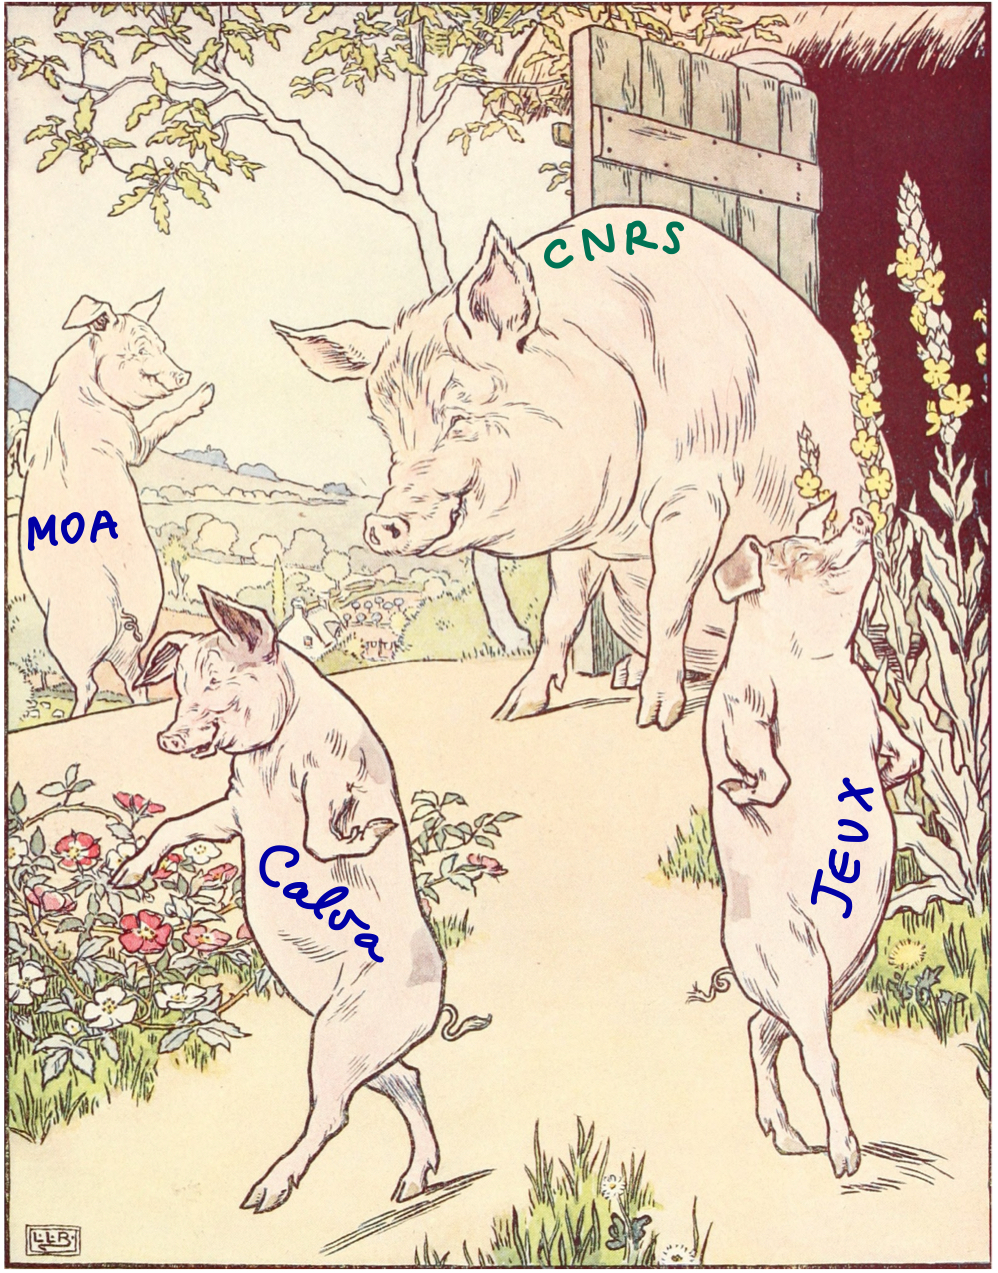
\includegraphics[height=5.0cm]{3-pigs}

\end{frame}

% Once upon a time...
\begin{frame}
\frametitle{\bf Once upon a time...}
\centering 
\includegraphics[width=.99\textwidth]{moa}
\end{frame}

% Once upon a time...
\begin{frame}
\frametitle{\bf Once upon a time...}
\centering 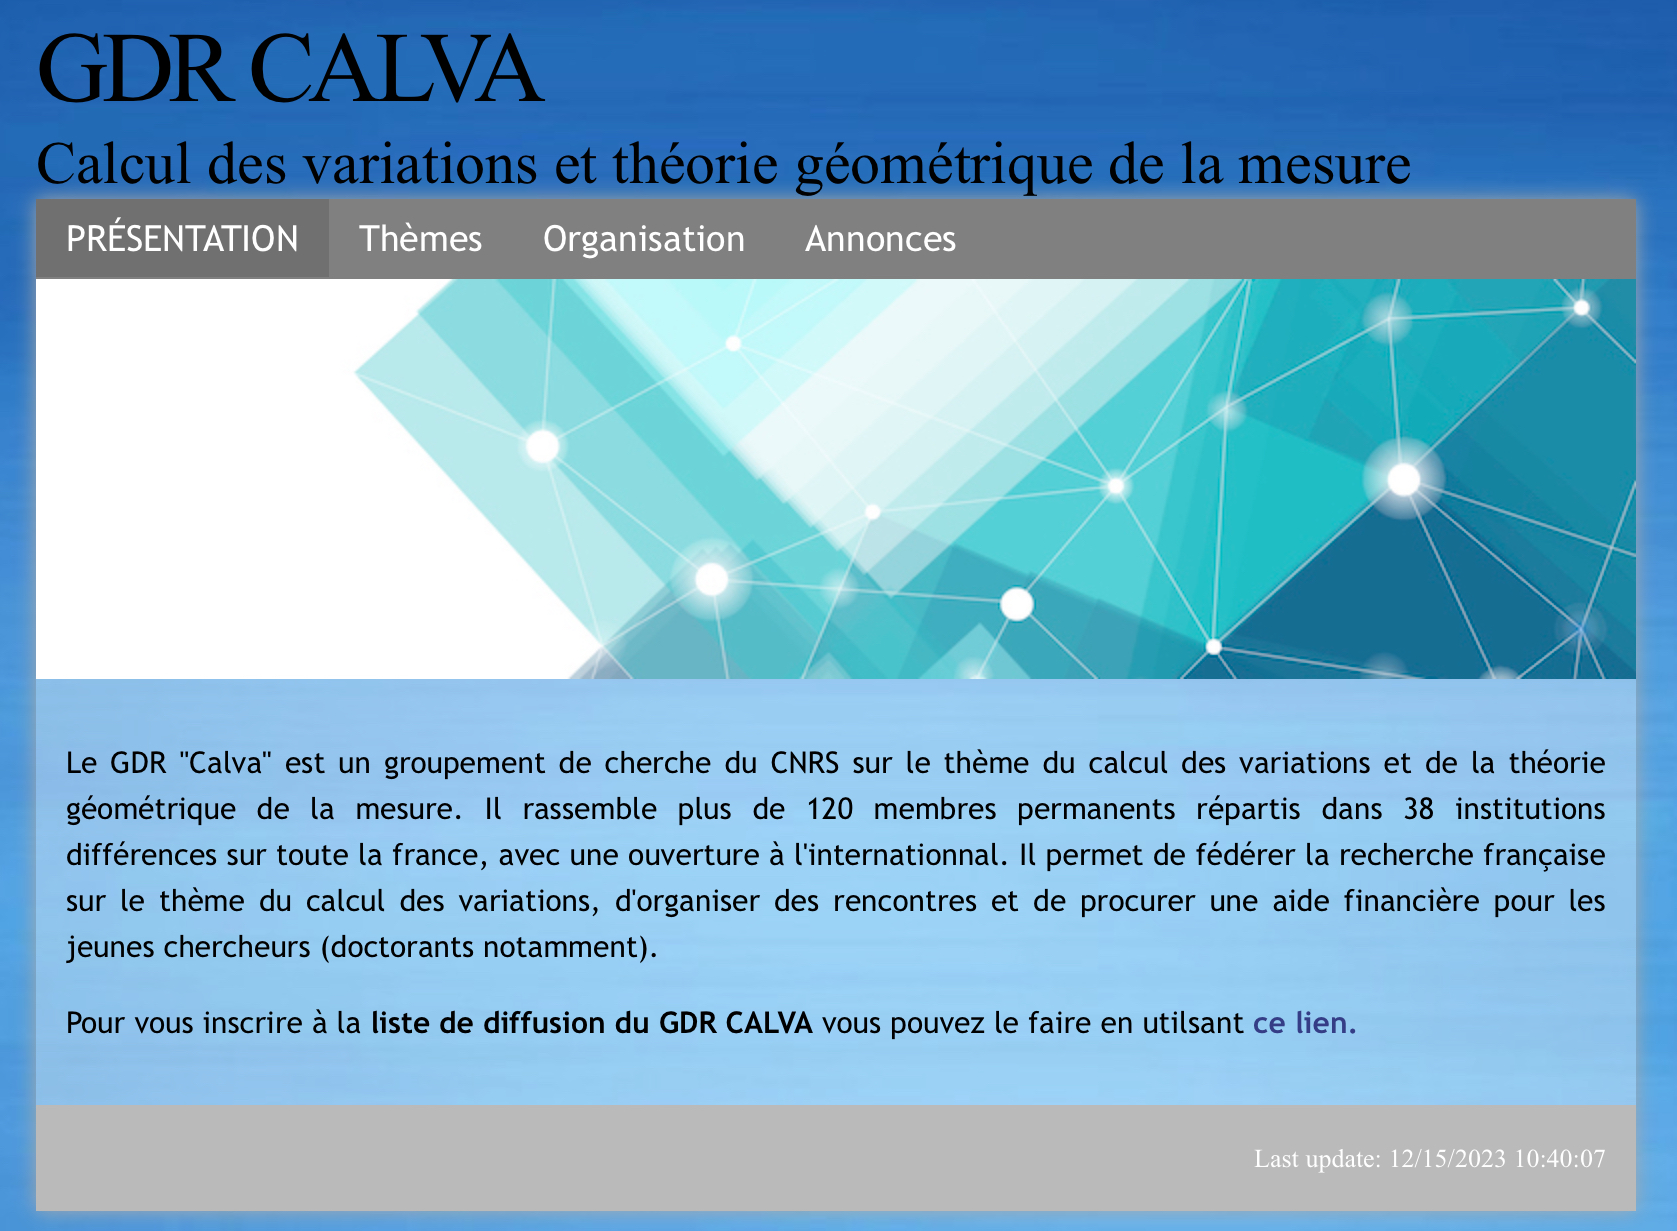
\includegraphics[width=.99\textwidth]{calva}
\end{frame}

% Once upon a time...
\begin{frame}
\frametitle{\bf Once upon a time...}
\centering 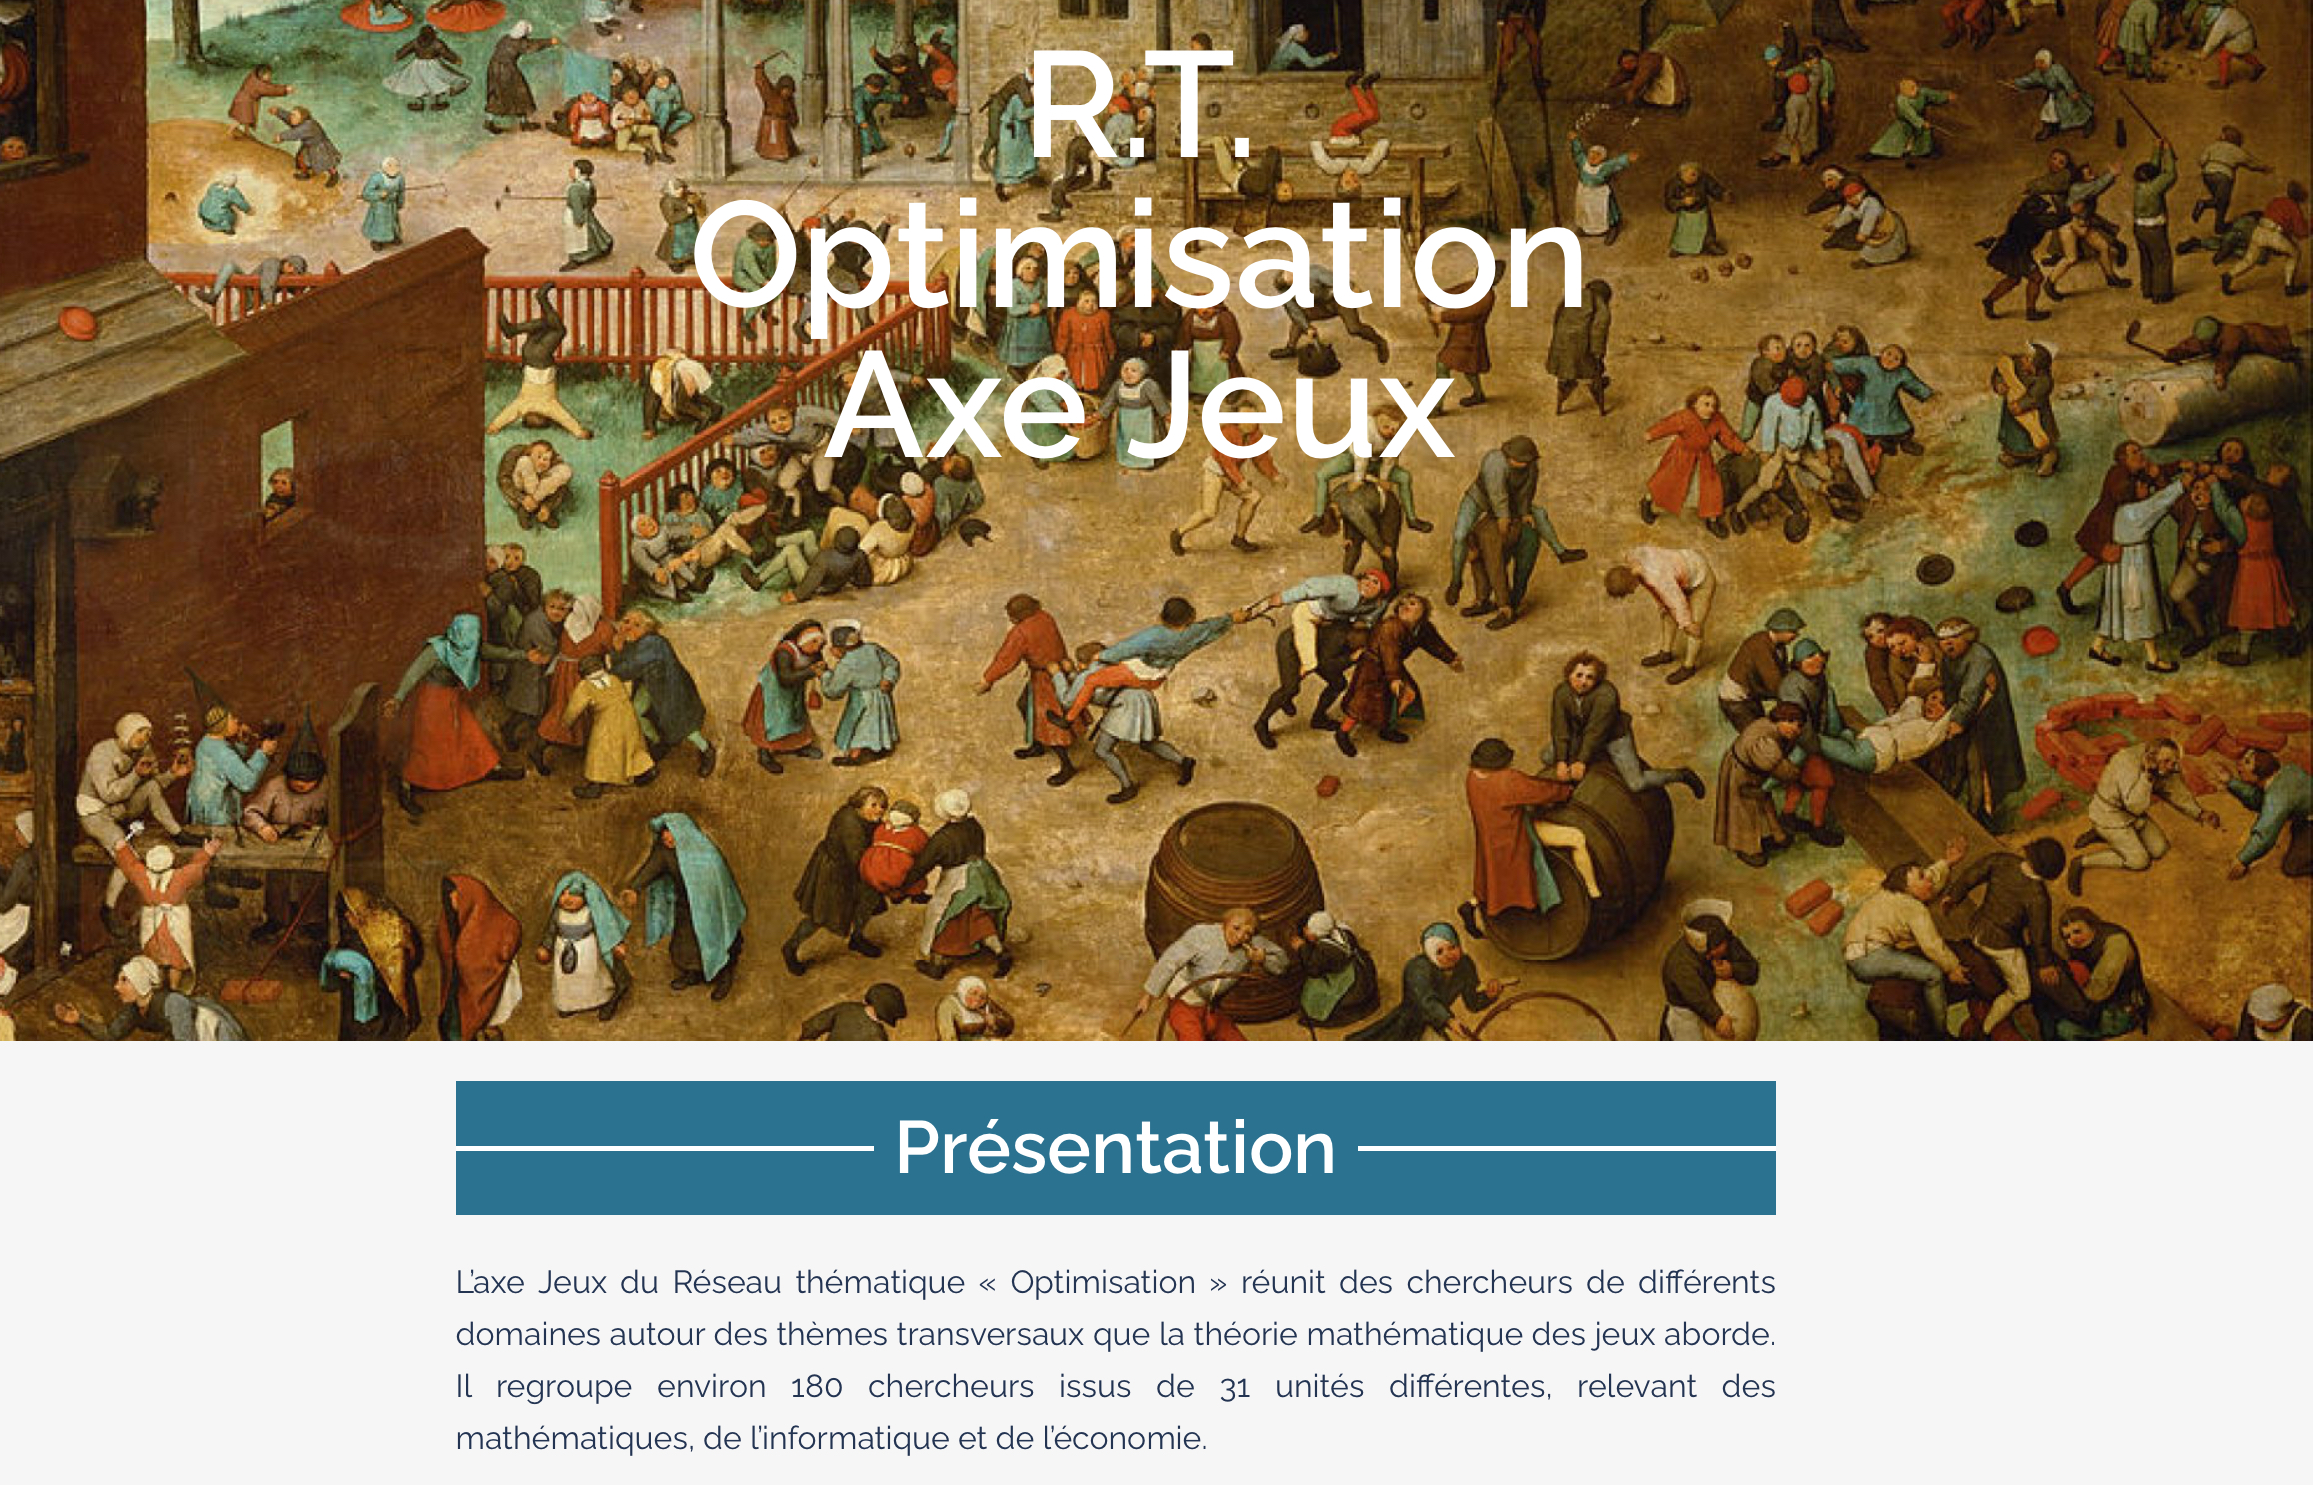
\includegraphics[width=.99\textwidth]{jeux}
\end{frame}

% Once upon a time...
\begin{frame}

\frametitle{\bf TA-DA}
\centering 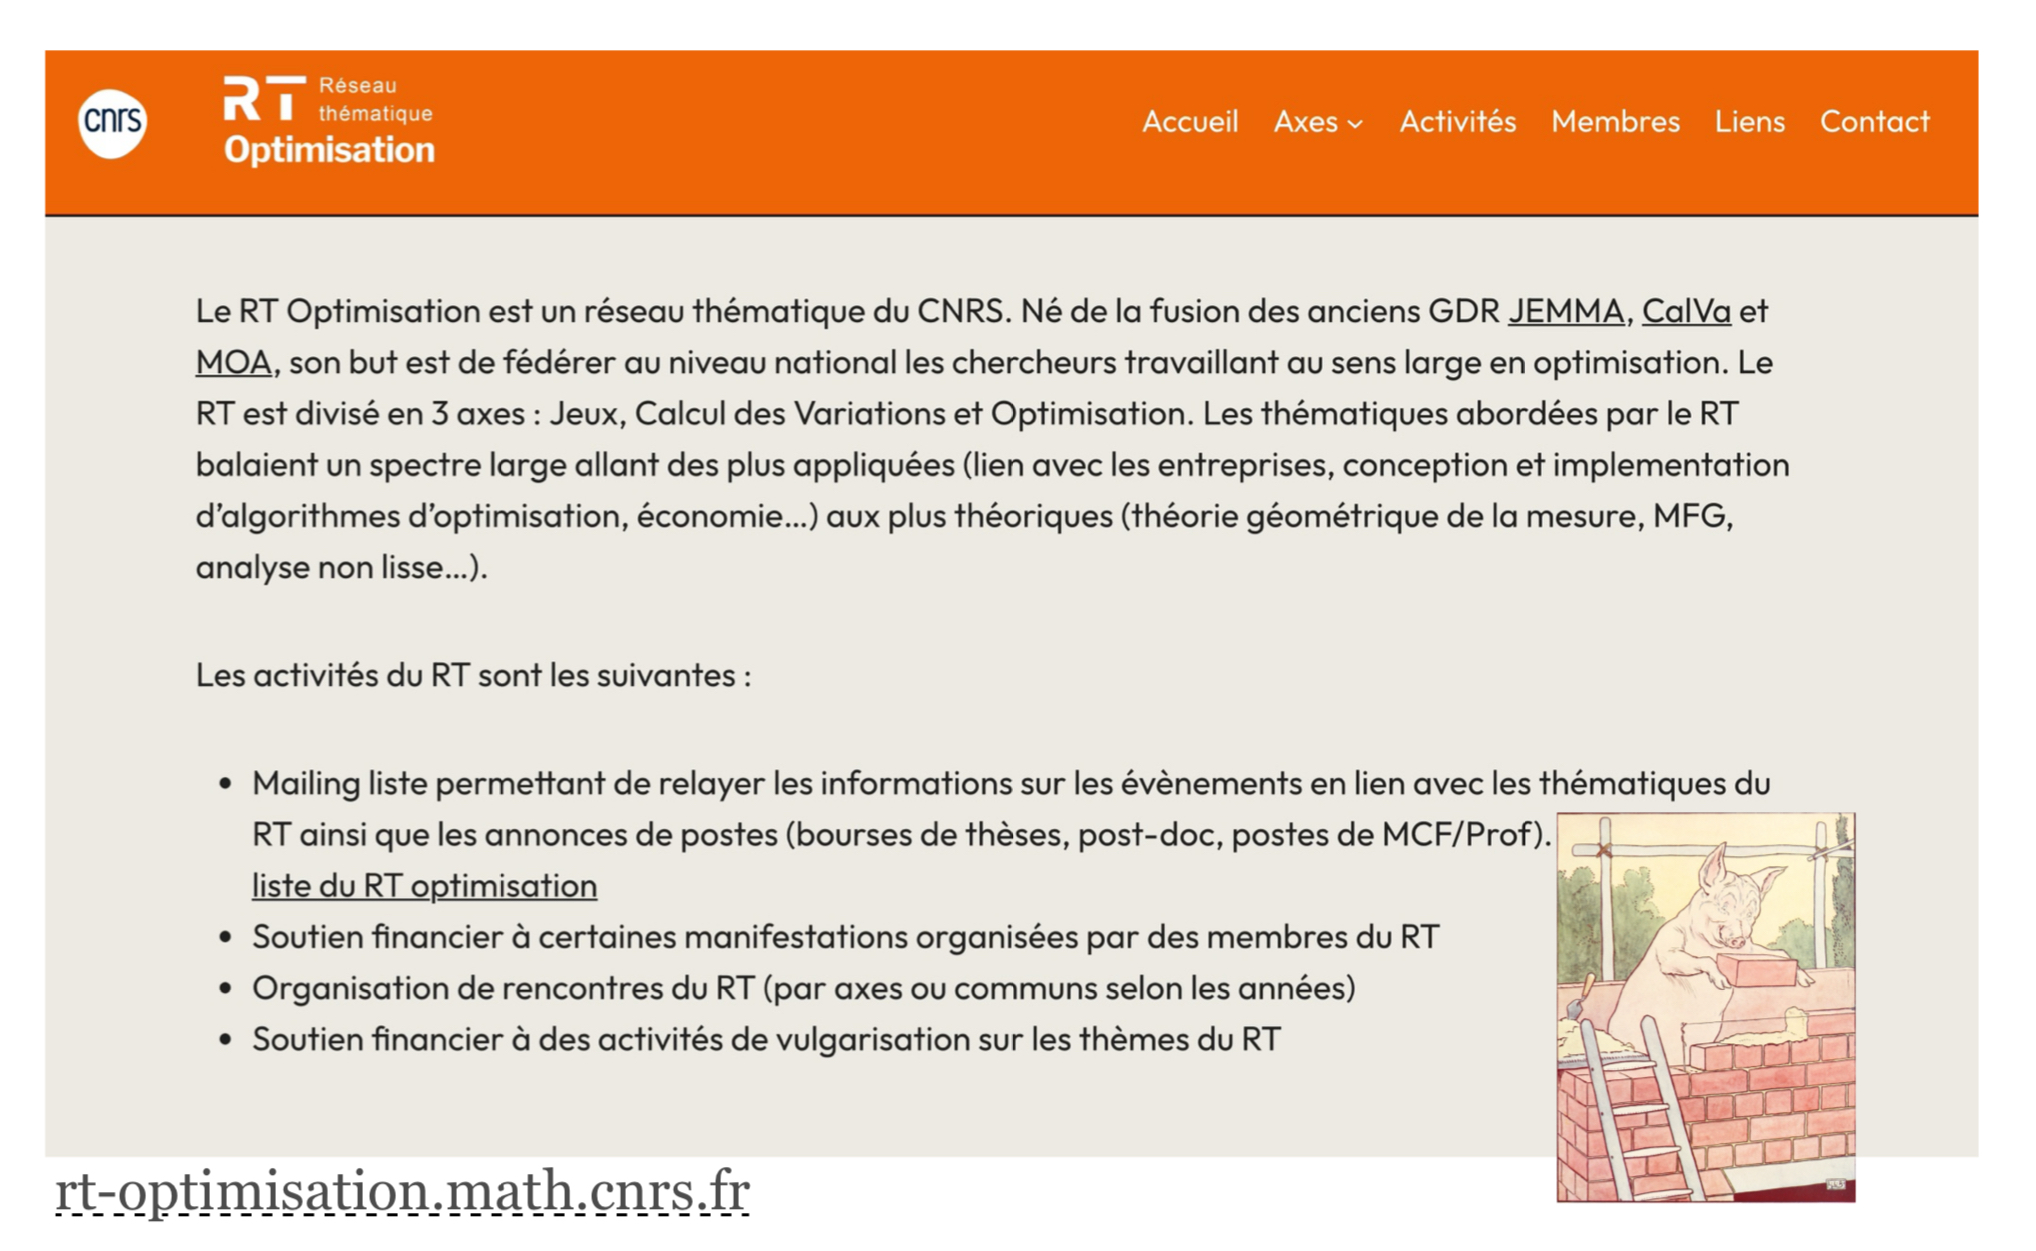
\includegraphics[width=.8\textwidth]{rt-opti}
\begin{itemize}
\item 1 RT (F. Santambrogio), 3 axes : MOA (M. Haddou), CalVa (M. Goldman), Jeux (C. Rainer)
\item Started 1st January 2024 (4 years), 50 Keuros/year
\item 300+ researchers, 50+ labs, 800+ mailing list subscribers (\texttt{rt-optimisation@listes.math.cnrs.fr})
\item Mostly maths, also computer science + economics
\item Funding events on optimisation
\end{itemize}

\end{frame}

% SMAI-MODE group on optimisation
\begin{frame}

\frametitle{\bf SMAI-MODE group on optimisation}
\centering 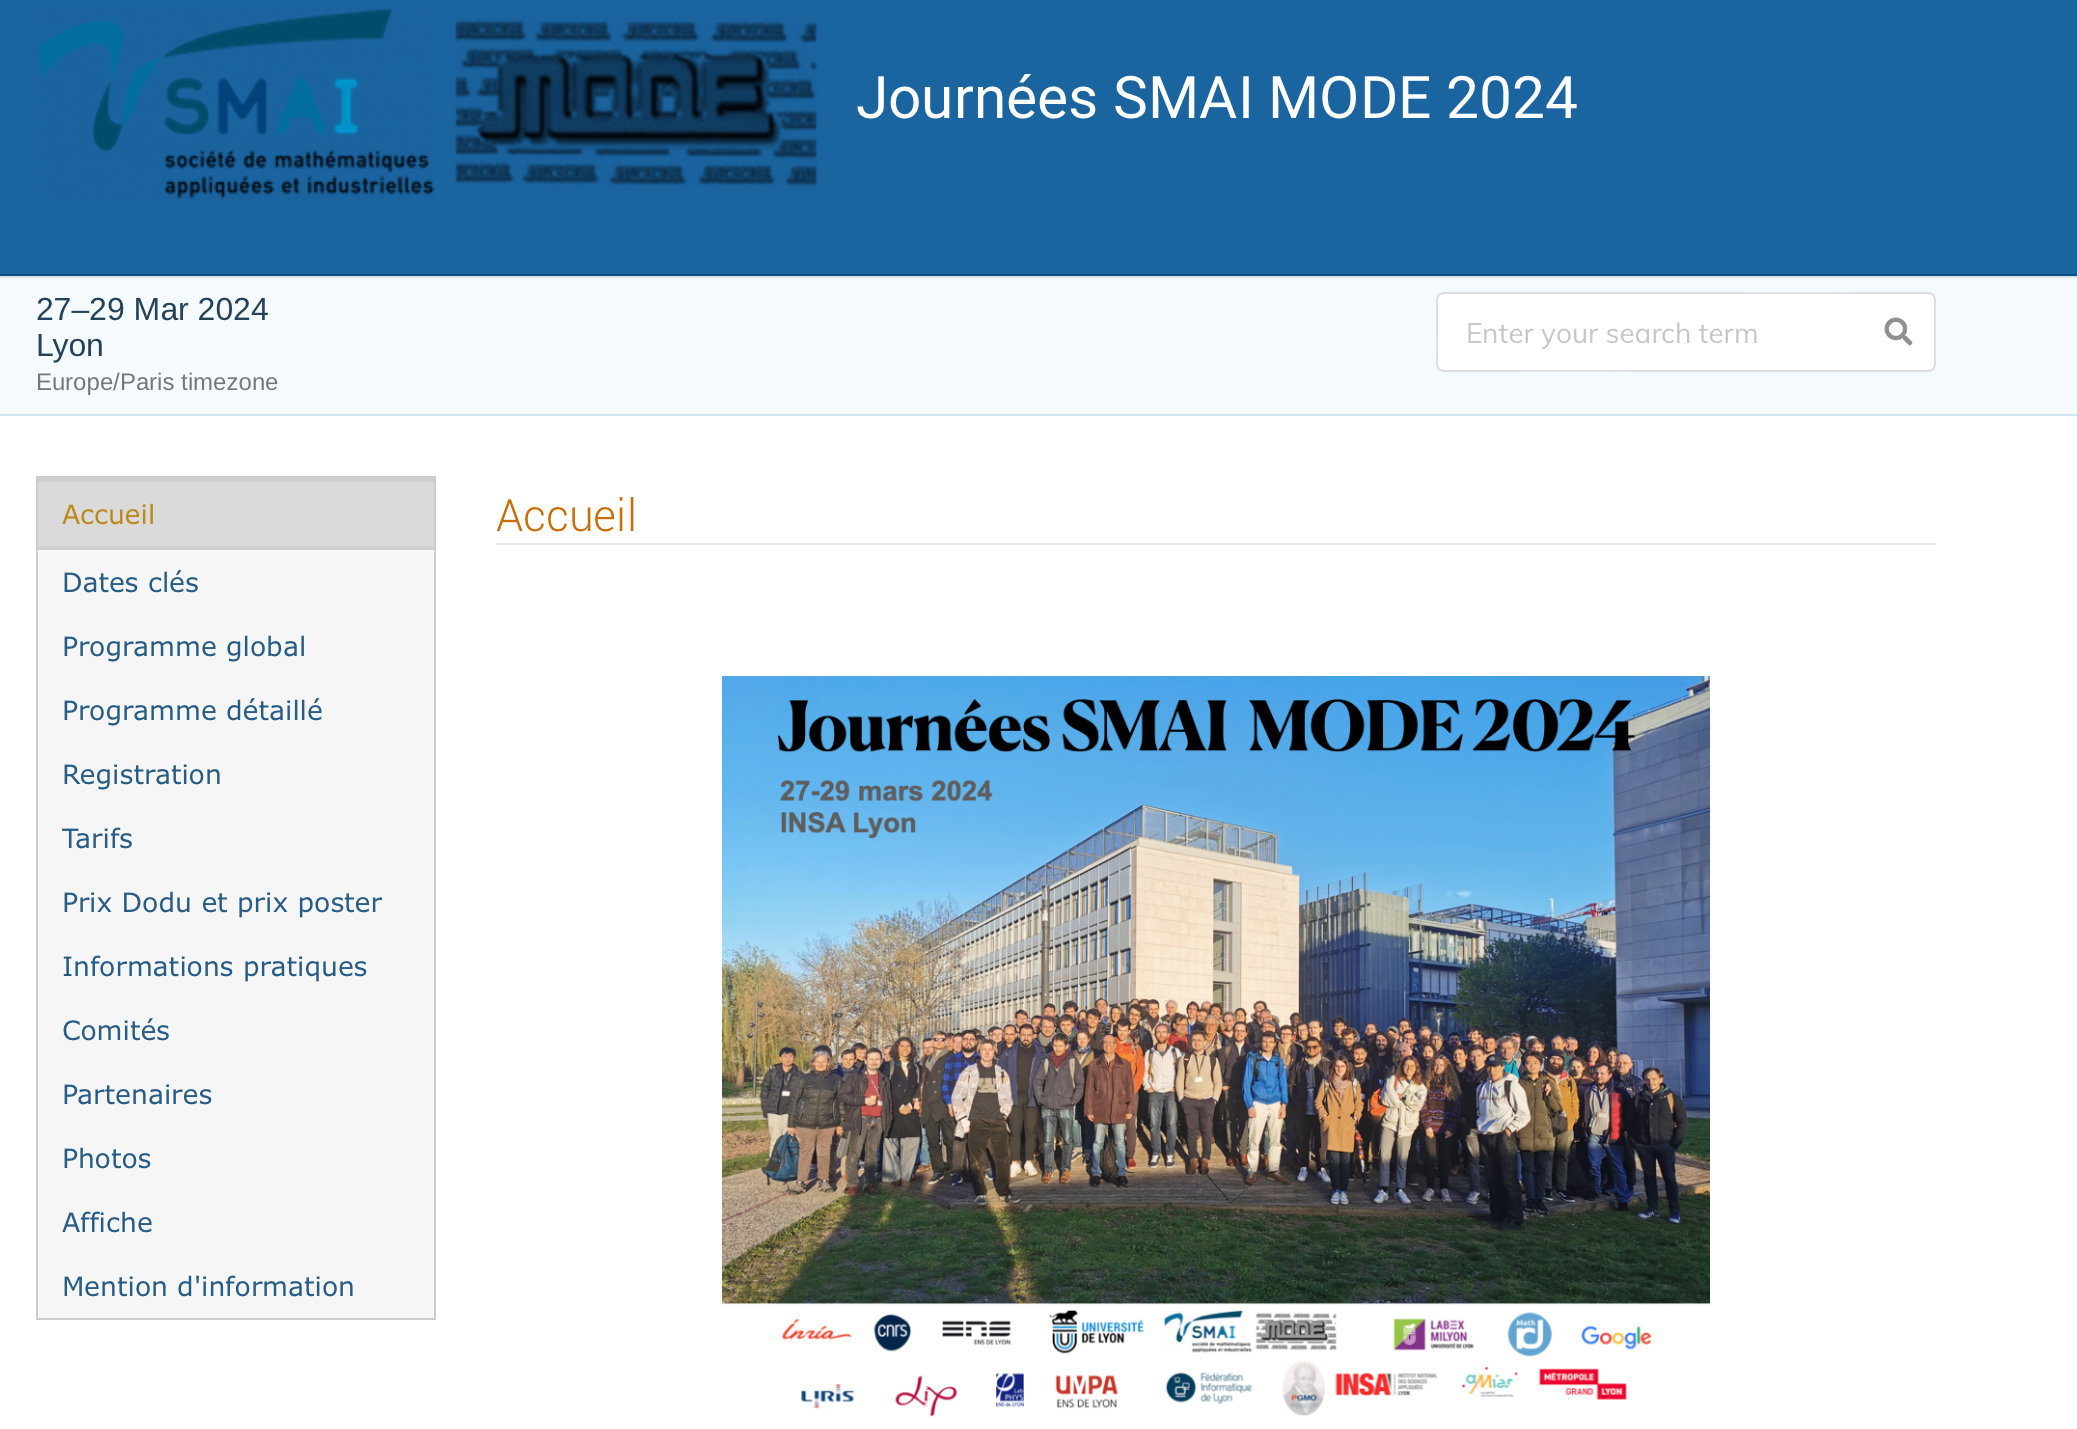
\includegraphics[width=.99\textwidth]{smai-mode}

\end{frame}

% Two more things
\begin{frame}
\frametitle{\bf Two more things}

\begin{itemize}
\item AI: there and back again (a journey into optimisation and control)
\item Efficient optimisation: algorithms, (sparse) numerical linear algebra and Automatic Differentiation (AD)
\end{itemize}

\centering 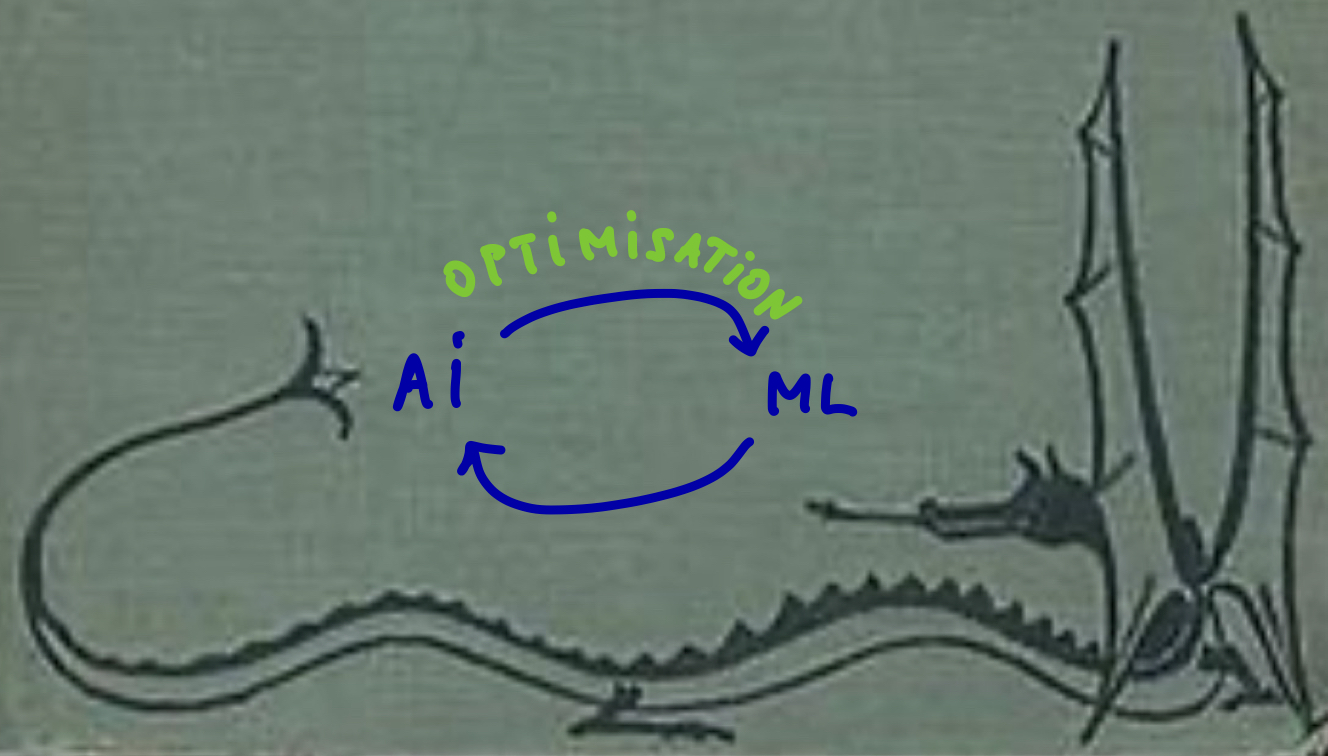
\includegraphics[width=.5\textwidth]{there-and-back}

\end{frame}

% ResNets as discretised linear control systems
\begin{frame}
\frametitle{\bf ResNets as discretised linear control systems}

After Agrachev (SISSA), Sarychev (Florence), Scagliotti (TUM) \emph{et al}:

\begin{itemize}
\item
  Agrachev, A. A.; Sarychev, A. V.
  \href{https://epubs.siam.org/doi/10.1137/19M1273049}{Control in the
  Spaces of Ensembles of Points}. \emph{SIAM J. Control Optim.}
  \textbf{58} (2020), no. 3, 1579--1596
\item
  Agrachev, A. A.; Sarychev, A. V.
  \href{https://link.springer.com/article/10.1007/s10883-021-09561-2}{Control
  on the Manifolds of Mappings with a View to the Deep Learning}.
  \emph{J. Dyn. Control Syst.} \textbf{28} (2021), 989--1008
\item
  A Scagliotti.
  \href{https://www.aimsciences.org/article/doi/10.3934/mcrf.2022036}{Deep
  Learning approximation of diffeomorphisms via linear-control systems}.
  \emph{MCRF} \textbf{13} (2023), no. 3, 1226-1257
\end{itemize}

\emph{ResNets} are compositions of nonlinear mappings

\[ \Phi = \Phi_M \circ \cdots \circ \Phi_1 \]

where $M$ is the depth of the neural network
and where each layer is of the form (additional term
\emph{wrt.} non-residual networks)

\[ \Phi_\ell(x) = x + \sigma(W_\ell+b_\ell). \]

\end{frame}

% ResNets as discretised linear control systems
\begin{frame}
\frametitle{\bf ResNets as discretised linear control systems}
For the approximation properties of such compositions see, \emph{e.g.},

\begin{itemize}
\item
  Yarotsky, D. \href{https://doi.org/10.1016/j.neunet.2017.07.002}{Error
  bounds for approximations with deep ReLU networks}. \emph{Neural
  Networks} \textbf{94} (2017), 103-114
\end{itemize}

in the case of non-residual networks. This composition can also be
interpretated as the explicit Euler discretisation of the \emph{Neural
ODE}

\[ \dot{x}(t) = \sigma(W(t)x(t)+b(t)), \]

where W and
b are now functions of time (continuum of
layers), \emph{controls}. Point of view developed, \emph{e.g.}, in
Tabuada \& Gharesifard:

\begin{itemize}
\item
  Tabuada, P.; Gharesifard, B.
  \href{https://arxiv.org/abs/2007.06007}{Universal Approximation Power
  of Deep Neural Networks via Nonlinear Control Theory}. arXiv:007.06007
  (2020)
\end{itemize}

See also \emph{constructive} approach for Lipschitz (ReLU-like)
activation function in references below:

\begin{itemize}
\item
  Li, Q.; Lin, T; Shen, Z.
  \href{https://ems.press/content/serial-article-files/32852}{Deep
  learning via dynamical systems: An approximation perspective}.
  \emph{J. Eur. Math. Soc.} \textbf{25} (2023), 1671--1709
\item
  Ruiz-Balet, D.; Zuazua, E.
  \href{https://epubs.siam.org/doi/10.1137/21M1411433}{Neural ode
  control for classification, approximation and transport}. \emph{SIAM
  Review} \textbf{65} (2022), no. 3, 735-773
\end{itemize}

\end{frame}

% ResNets as discretised linear control systems
\begin{frame}
\frametitle{\bf ResNets as discretised linear control systems}

\textbf{Alternative point of view.} Nonlinear in the data
x but \emph{linear} in the parameters:

\[ \Phi_\ell(x) = x + G(x)u_\ell. \]

Composition now interpretated as the discretisation of

\[ \dot{x}(t) = G(x(t))u(t) = \sum_{i=1}^m u_i(t)F_i(x(t)) \]

where the \emph{smooth} vector fields $F_1,\ldots,F_m$
are the columns of the nonlinear function $G$.\\
\ \\
Ability to learn data (finite or \emph{continuum}) = controllability
properties of the control system for \emph{ensembles}.

\end{frame}

% Ensembles
\begin{frame}
\frametitle{\bf Ensembles}

\textbf{Definition.} For $\Theta$ compact
subset of $\R^n$ (set of possibly infinite indices of the data), define an ensemble as a continuous
\emph{injective} map from $\Theta$ to
$\R^n$. Denote $\mathscr{E}_\Theta$ the set of ensembles.\\
\ \\
\textbf{Example.} For $|\Theta| = N < \infty$ finite, ensemble = open subset of $(\R^n)^N$ made of
pairwise distinct vectors: $(x_1,\ldots,x_N) \in (\R^n)^{(N)}$.

\centering 
\includegraphics[height=6.0cm]{conf-icerm}

\end{frame}

% Exact controllability
\begin{frame}
\frametitle{\bf Exact controllability}

For an admissible control u in
$L^2([0,1],\R^m)$ (+ growth conditions on vector fields), define the time $1$ flow $\Phi_u$
of the controlled system

\[ \dot{x}(t) = \sum_{i=1}^m u_i(t)F_i(x(t)) \qquad (1) \]

mapping an initial condition $x_0$ to $\Phi_u(x_0) := x(1,u,x_0)$.\\
\ \\
\textbf{Definition.} The control system (1) is said to be controllable
on $\mathscr{E}_\Theta$ if, for any ensembles $\gamma_0$, $\gamma_f$, there exists an admissible
control $u$ \emph{s.t.}

\[ \Phi_u \circ \gamma_0 = \gamma_f. \]

\textbf{Example.} For $|\Theta| = N$ finite and any ensembles 
$(x^0_1,\ldots,x^0_N)$, $(x^f_1,\ldots,x^f_N)$ in
$(\R^n)^{(N)}$, controllability means that there exists an admissible control
$u$ \emph{s.t.}

\[ \Phi_u(x^0_j) = x^f_j,\quad j=1,\ldots,N. \]

\textbf{Theorem.} (Agrachev-Sarychev'2020) For $m \geq 2$ controls, any $N \geq 1$ and $k$ sufficiently
large, the set of vector fields $F_1,\ldots,F_m$
\emph{s.t.} controllability holds on $\mathscr{E}_\Theta$ with $|\Theta| = N$, is residual in
$\mathscr{C}^k(\R^n)$.
%% \ \\
%% \textbf{Remark.} Typical control-geometric proof: for \emph{generic}
%% vector fields $F_1,\ldots,F_m$, the
%% family of folds $F^{(N)}_1,\ldots,F^{(N)}_m$ is bracket generating on $(\R^n)^{(N)}$:
%%  
%% \[ \text{Lie}_{x^{(N)}} \lbrace F^{(N)}_1,\ldots,F^{(N)}_m \rbrace = (\R^n)^N,\quad x^{(N)} \in (\R^n)^{(N)}, \]
%%  
%% where the \emph{fold} of vector field $F$ is
%% $F^{(N)}(x_1,\ldots,x_N) := (F(x_1),\ldots,F(x_N))$. Controllability then ensured
%% by Chow-Rashewsky.
  
\end{frame}

% Approximate reachability
\begin{frame}
\frametitle{\bf Approximate reachability}

\textbf{Definition.} Let $\gamma_0$ and $\gamma_f$ be two ensembles in
$\mathscr{E}_\Theta$. Then $\gamma_f$ is said to be $\mathscr{C}^0$-\emph{approximately
reachable} from $\gamma_0$ by control system (1) if, for any $\varepsilon > 0$, there exists an admissible control
$u$ \emph{s.t.}

\[ \sup_{\theta \in \Theta} |\Phi_u(\gamma_0(\theta))-\gamma_f(\theta)| \leq \varepsilon. \]

\textbf{Remark.} As a flow, any such $\Phi_u$ is diffeotopic to identity since

\[ x(0,u,\cdot) = \text{Id},\quad x(1,u,\cdot) = \Phi_u. \]

So if $\gamma_f$ is reachable from $\gamma_0$, the two ensembles must be diffeotopic.

\end{frame}

% Approximate reachability
\begin{frame}
\frametitle{\bf Approximate reachability}

\textbf{Definition.} The family $F_1,\ldots,F_m$ satisfies the \emph{(Lie
algebra) strong approximation property} if there exists $k
\geq 1$ \emph{s.t.}, for any $\mathscr{C}^k$ vector field $X$ and for any compact $K
\subset \R^n$, there is $\delta > 0$ \emph{s.t.}

\[ \inf \lbrace \max_{x \in K} |X(x)-Y(x)| \text{ with } Y \in \text{Lie} \lbrace  F_1,\ldots,F_m \rbrace,\ \Vert Y \Vert_{1,K} \leq \delta \rbrace = 0. \]

\textbf{Remark.} The strong approximation property implies that, for
every $N \geq 1$, the folds of $F_1,\ldots,F_m$ are bracket generating on
$(\R^n)^{(N)}$. So (exact) controllability holds for finite sets $\Theta$.\\
\ \\
\textbf{Example.} The family below satisfies the strong approximation
property $(n \geq 2)$:

\[ F_i(x) = \frac{\partial}{\partial x_i}\quad 
  G_i(x) = e^{-|x|^2} \frac{\partial}{\partial x_i}\quad i=1,\ldots,n. \]

\textbf{Theorem.} (Agrachev-Sarychev'2021) Let $\gamma_0$ and $\gamma_f$ be two \emph{diffeotopic}
ensembles in $\mathscr{E}_\Theta$. Under the strong approximation property, $\gamma_f$
is $\mathscr{C}^0$-\emph{approximately reachable} from $\gamma_0$ by control system (1).\\

\end{frame}

% A glimpse of AD 
\begin{frame}
\frametitle{\bf A glimpse of AD}
\begin{itemize}
\item Good optimisation needs good gradients (+ Hessians)
\item More or less built-in with modern languages / optimisation modellers
\item Work at LLVM level (Enzyme)
\item Sparse AD: graph coloring techniques
\end{itemize}

\centering 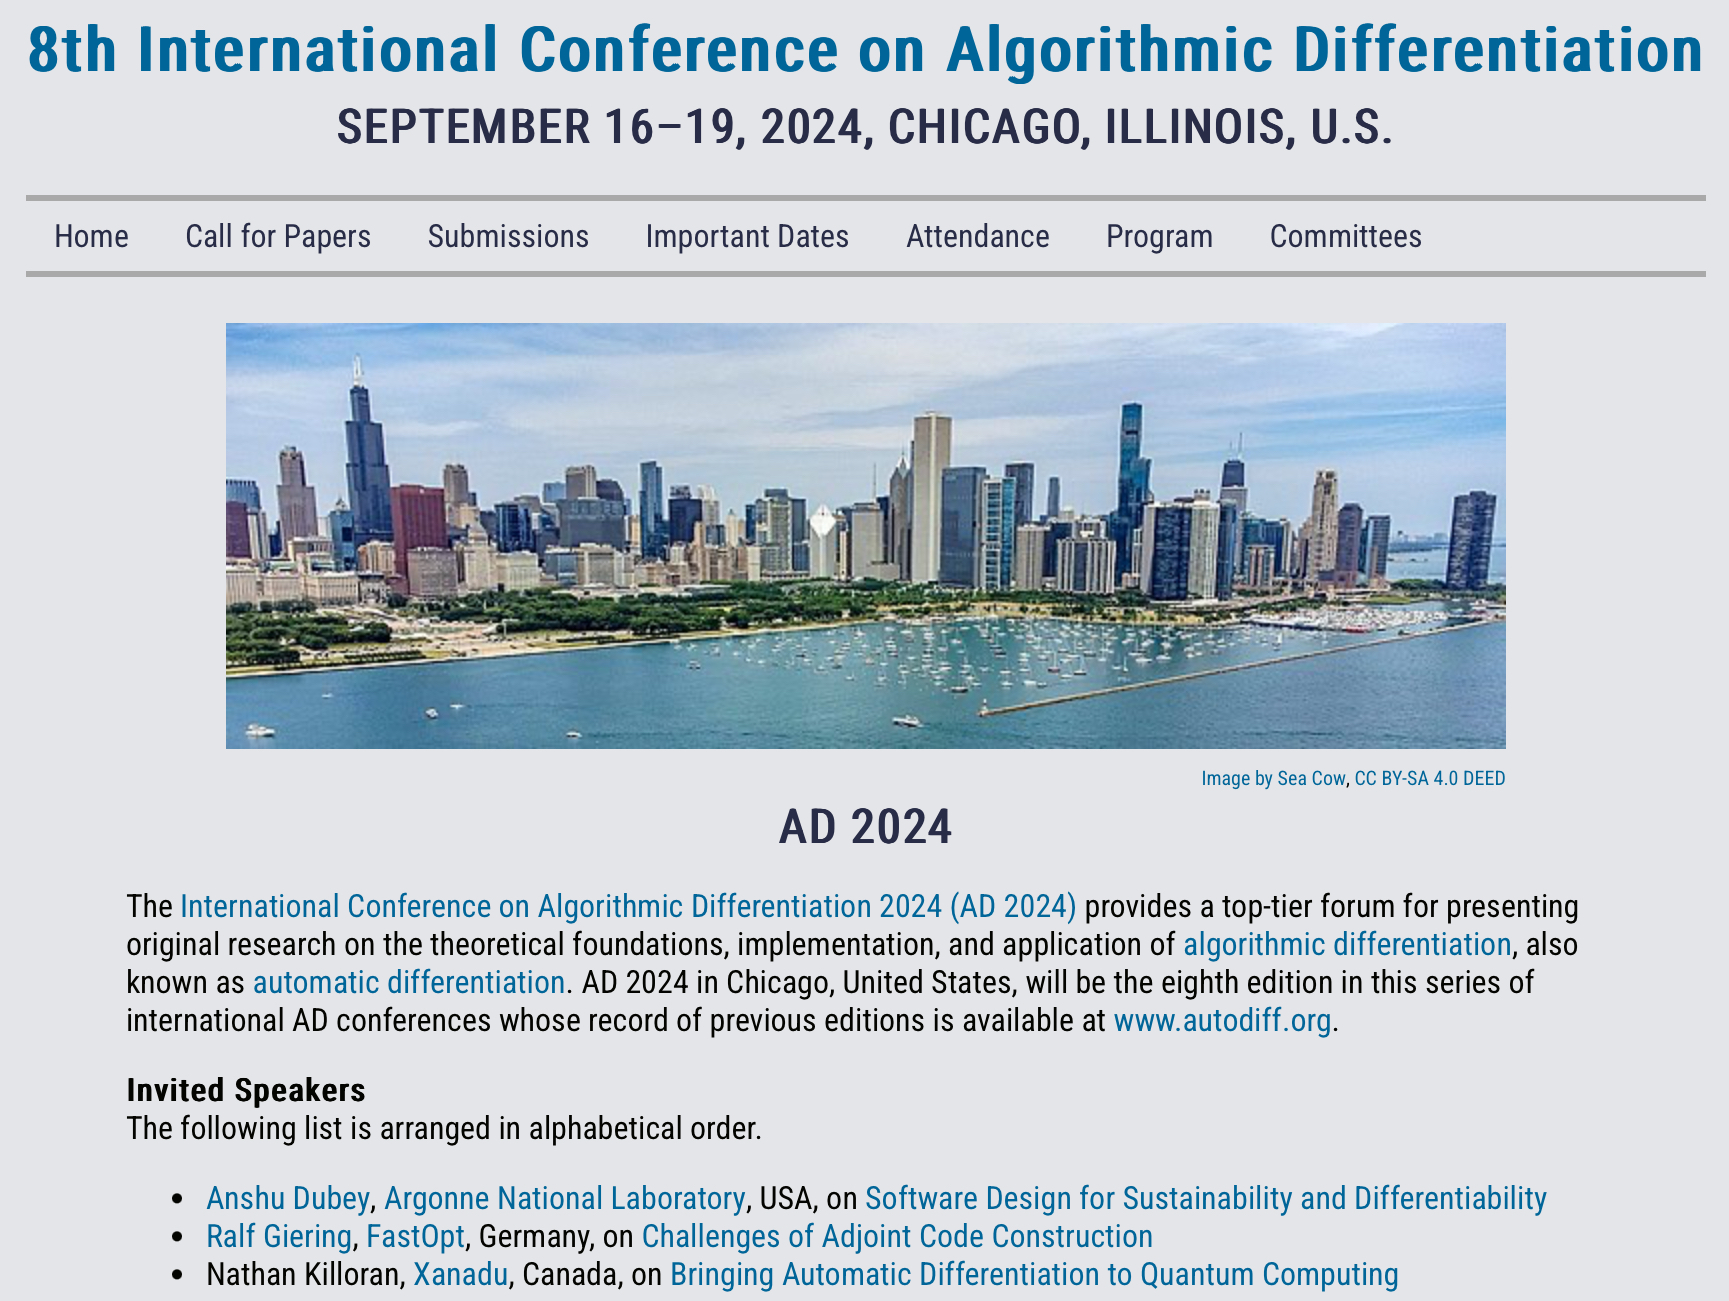
\includegraphics[height=6.0cm]{ad2024}

\end{frame}

% A glimpse of AD 
\begin{frame}
\frametitle{\bf A glimpse of AD}

$$ y = f(x_1, x_2) = \sin x_1 + x_1 x_2 $$

\centering 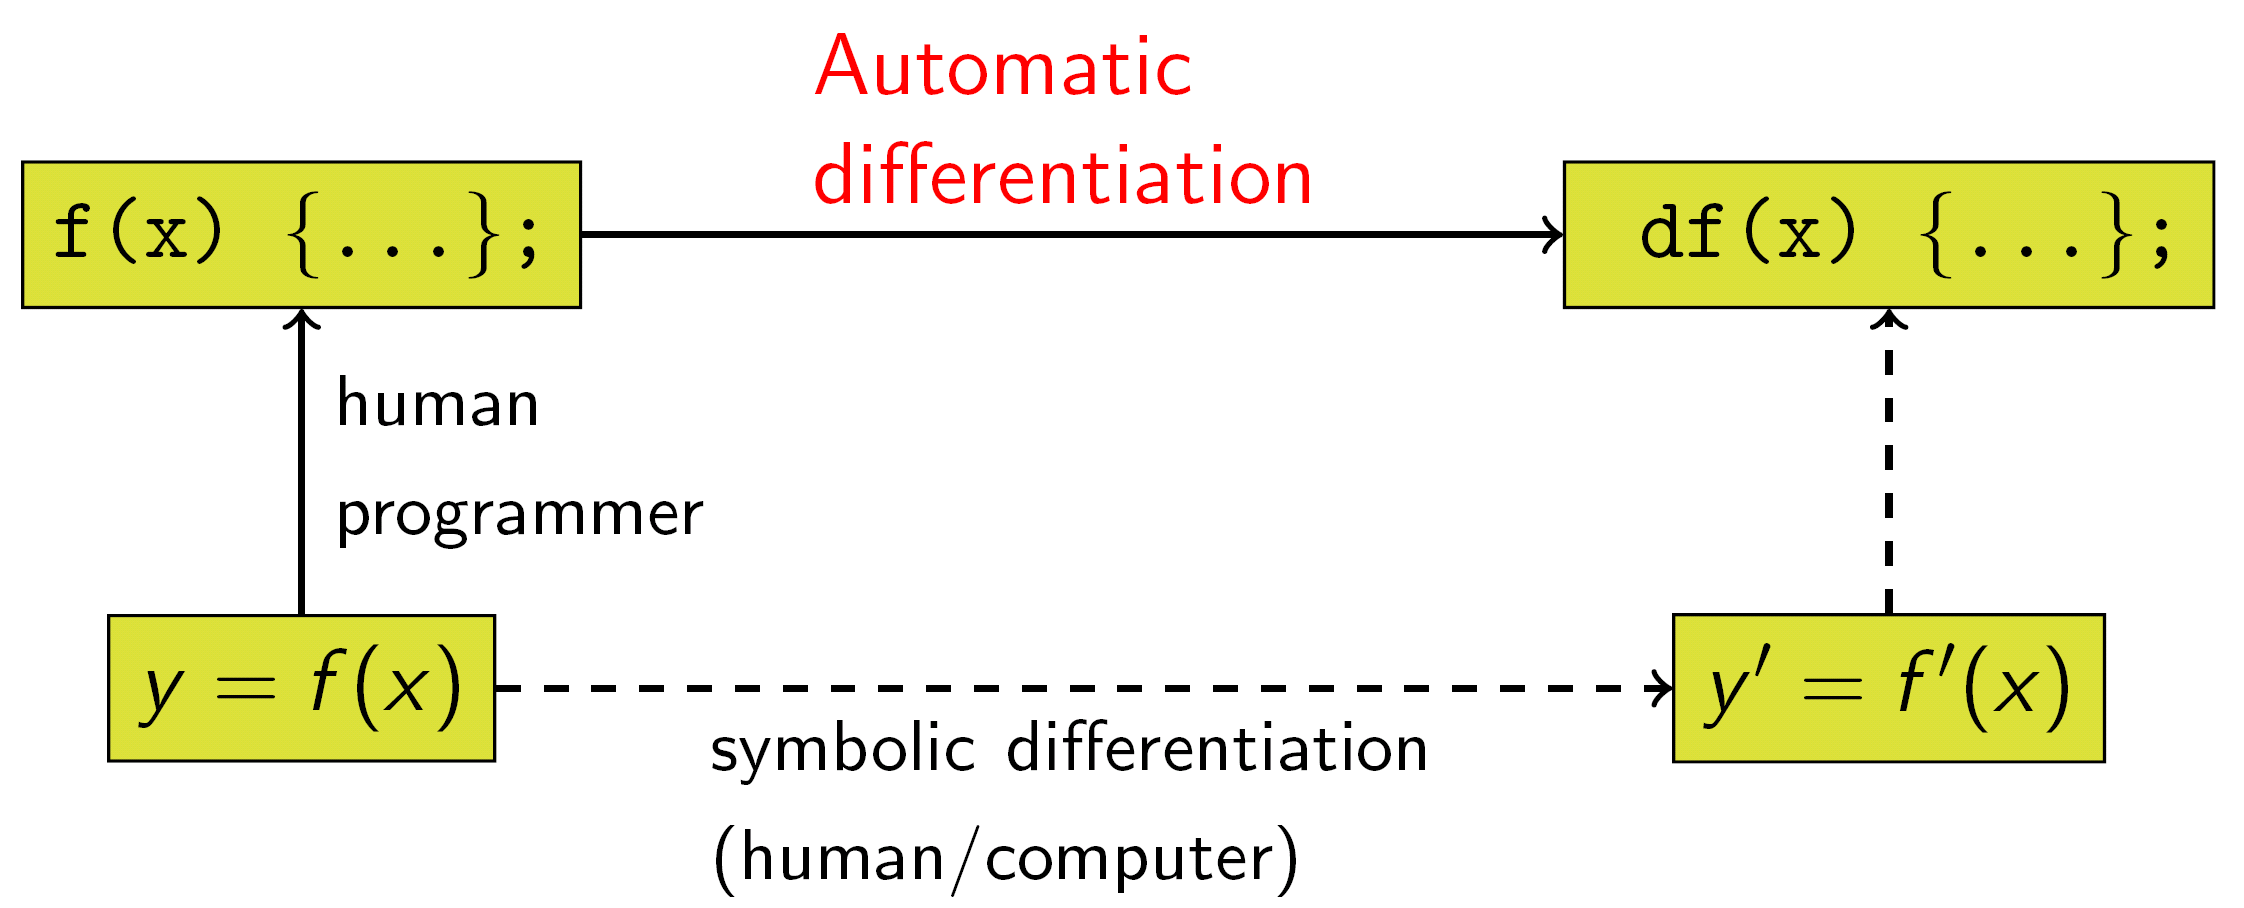
\includegraphics[width=0.7\textwidth]{ad}

\hspace*{-0.7cm} 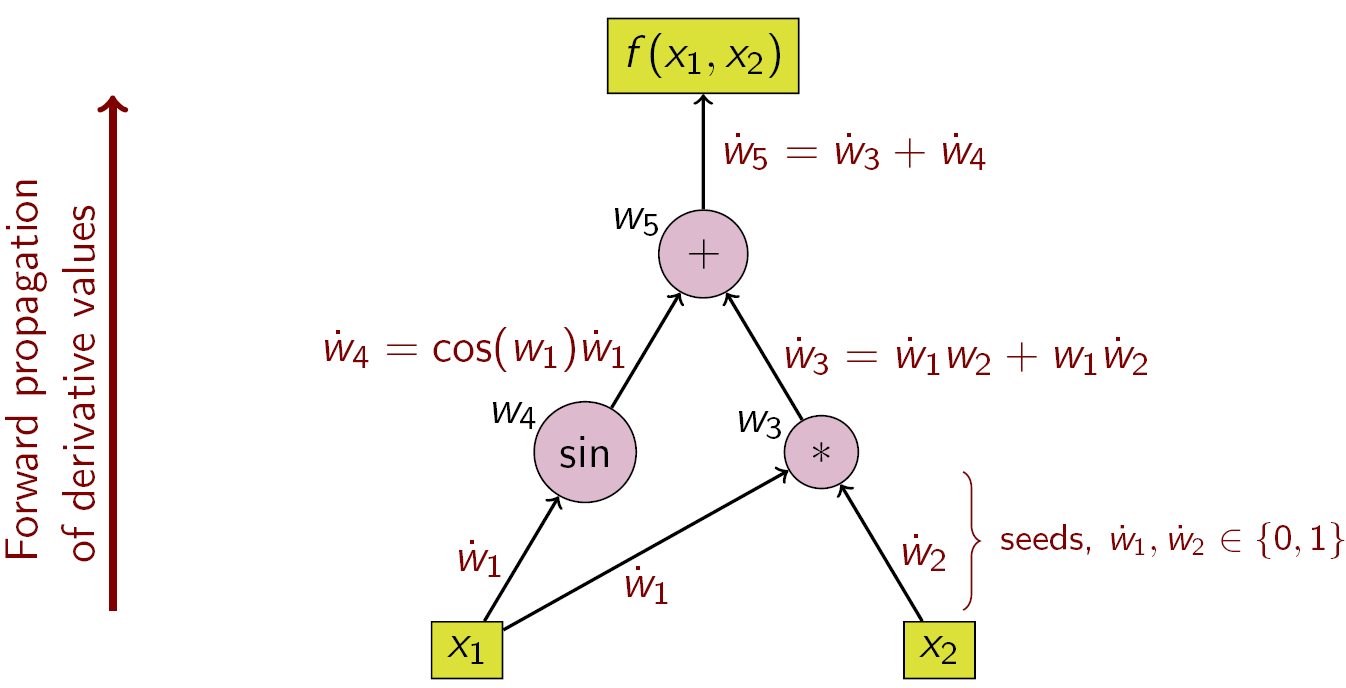
\includegraphics[width=0.55\textwidth]{forward} 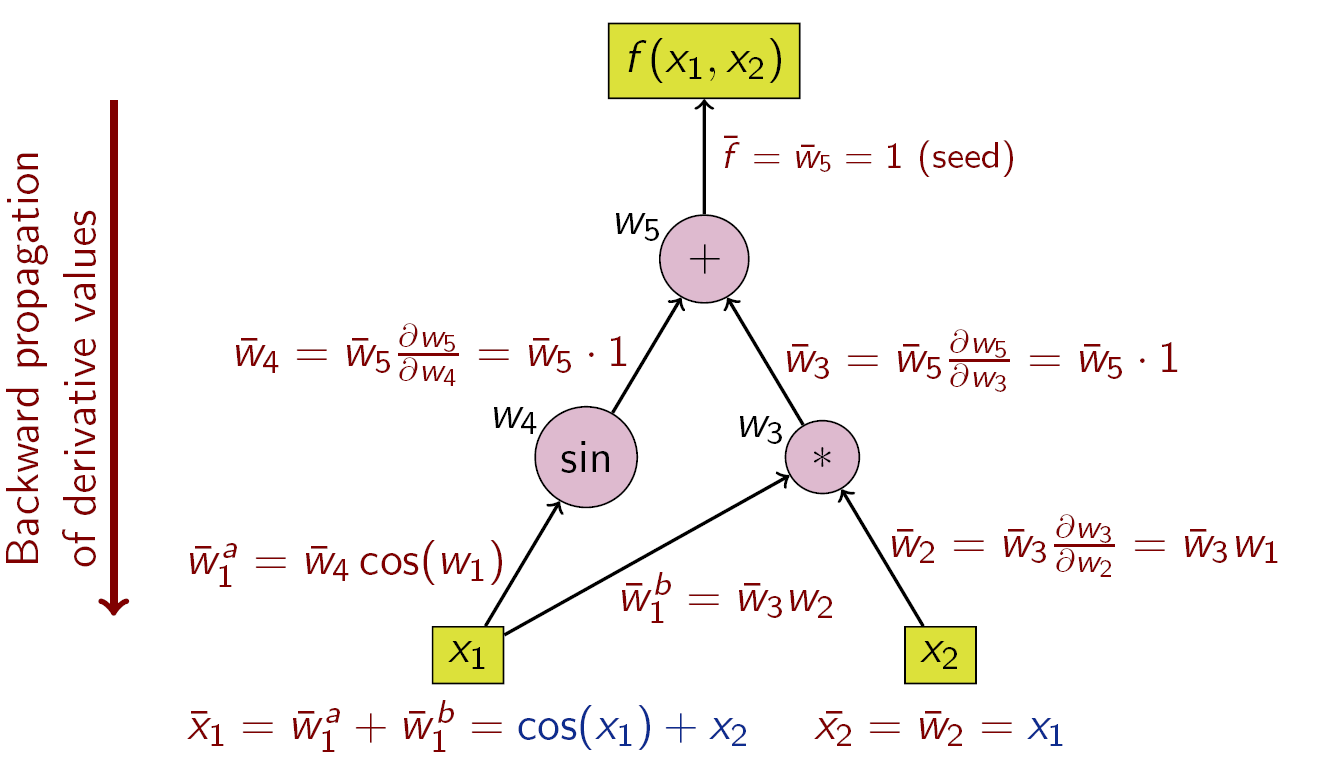
\includegraphics[width=0.55\textwidth]{reverse}

\begin{flushright}
Source: Wikipedia on AD
\end{flushright}

\end{frame}

% Optimisation modellers: finite dim
\begin{frame}
\frametitle{\bf Optimisation modellers: finite dim}

\centering 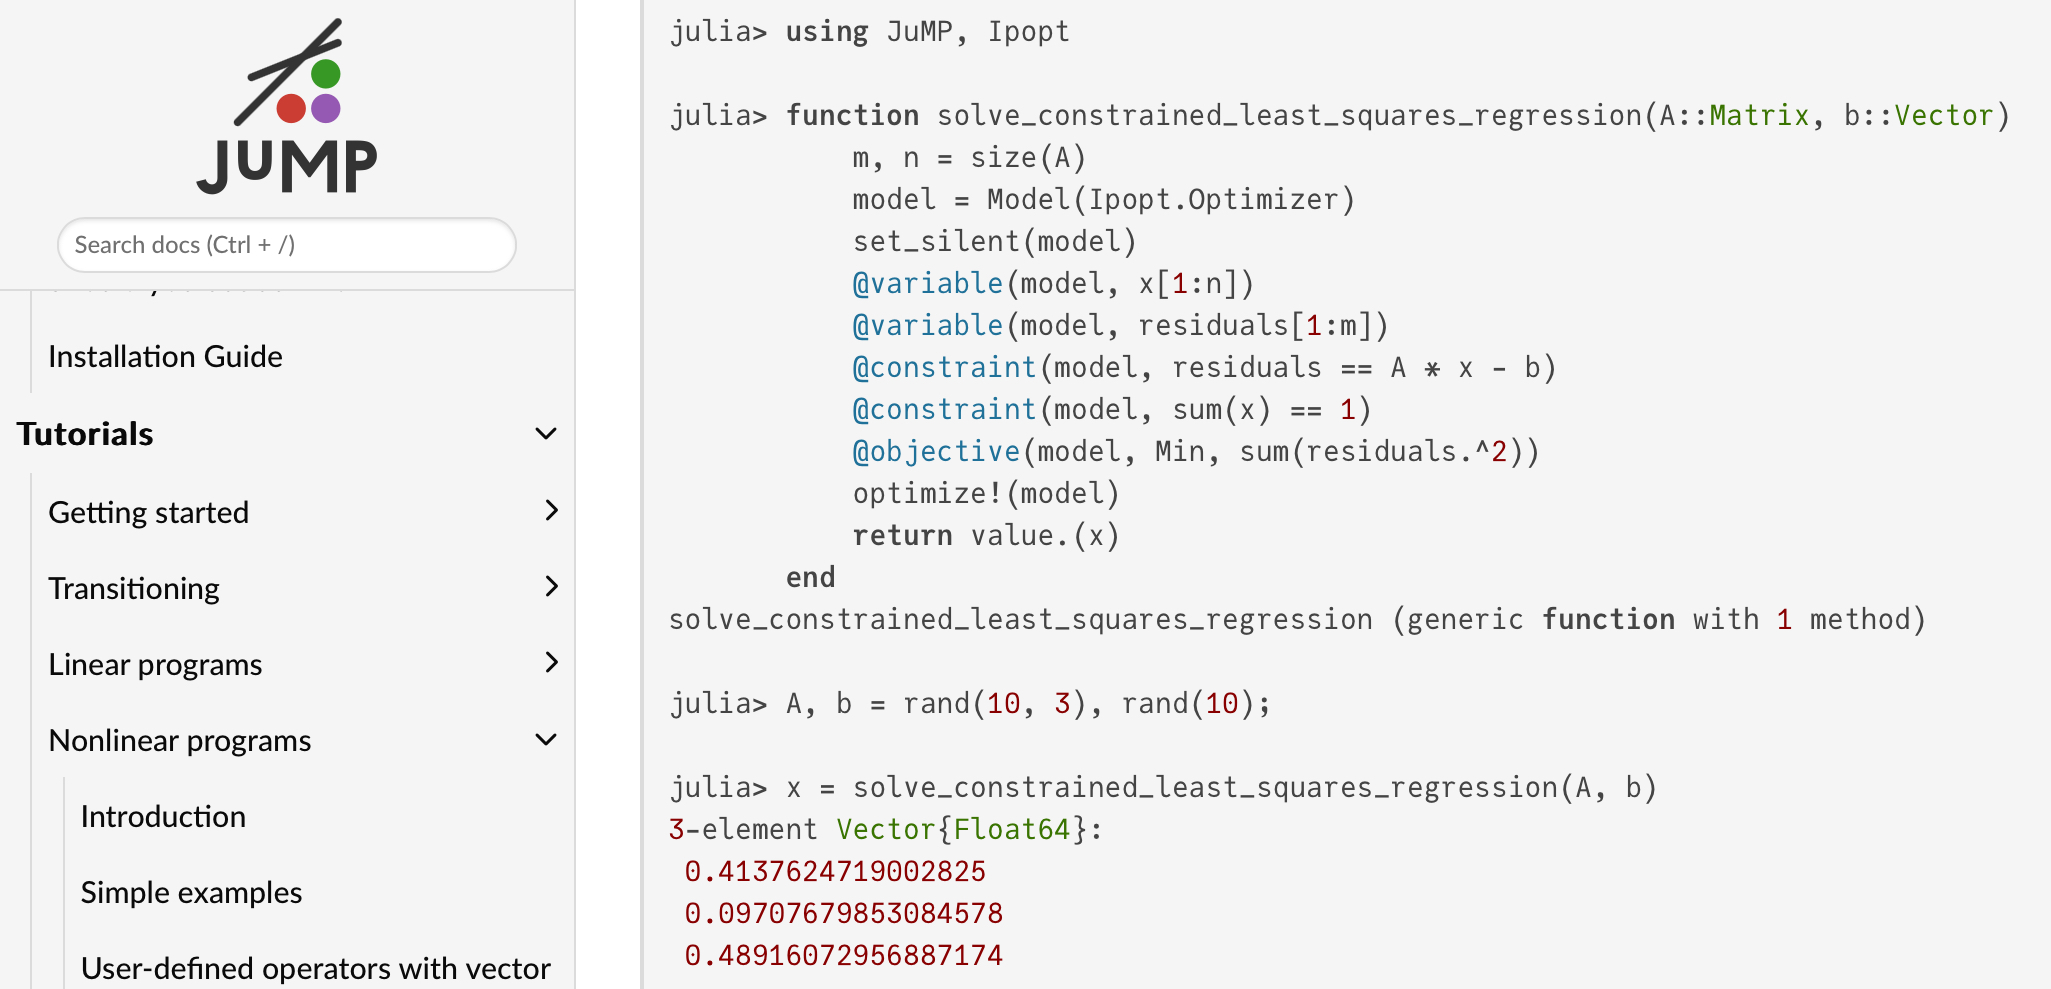
\includegraphics[width=1.05\textwidth]{jump}

\end{frame}

% Optimisation modellers: finite dim
\begin{frame}
\frametitle{\bf Optimisation modellers: finite dim}

\centering 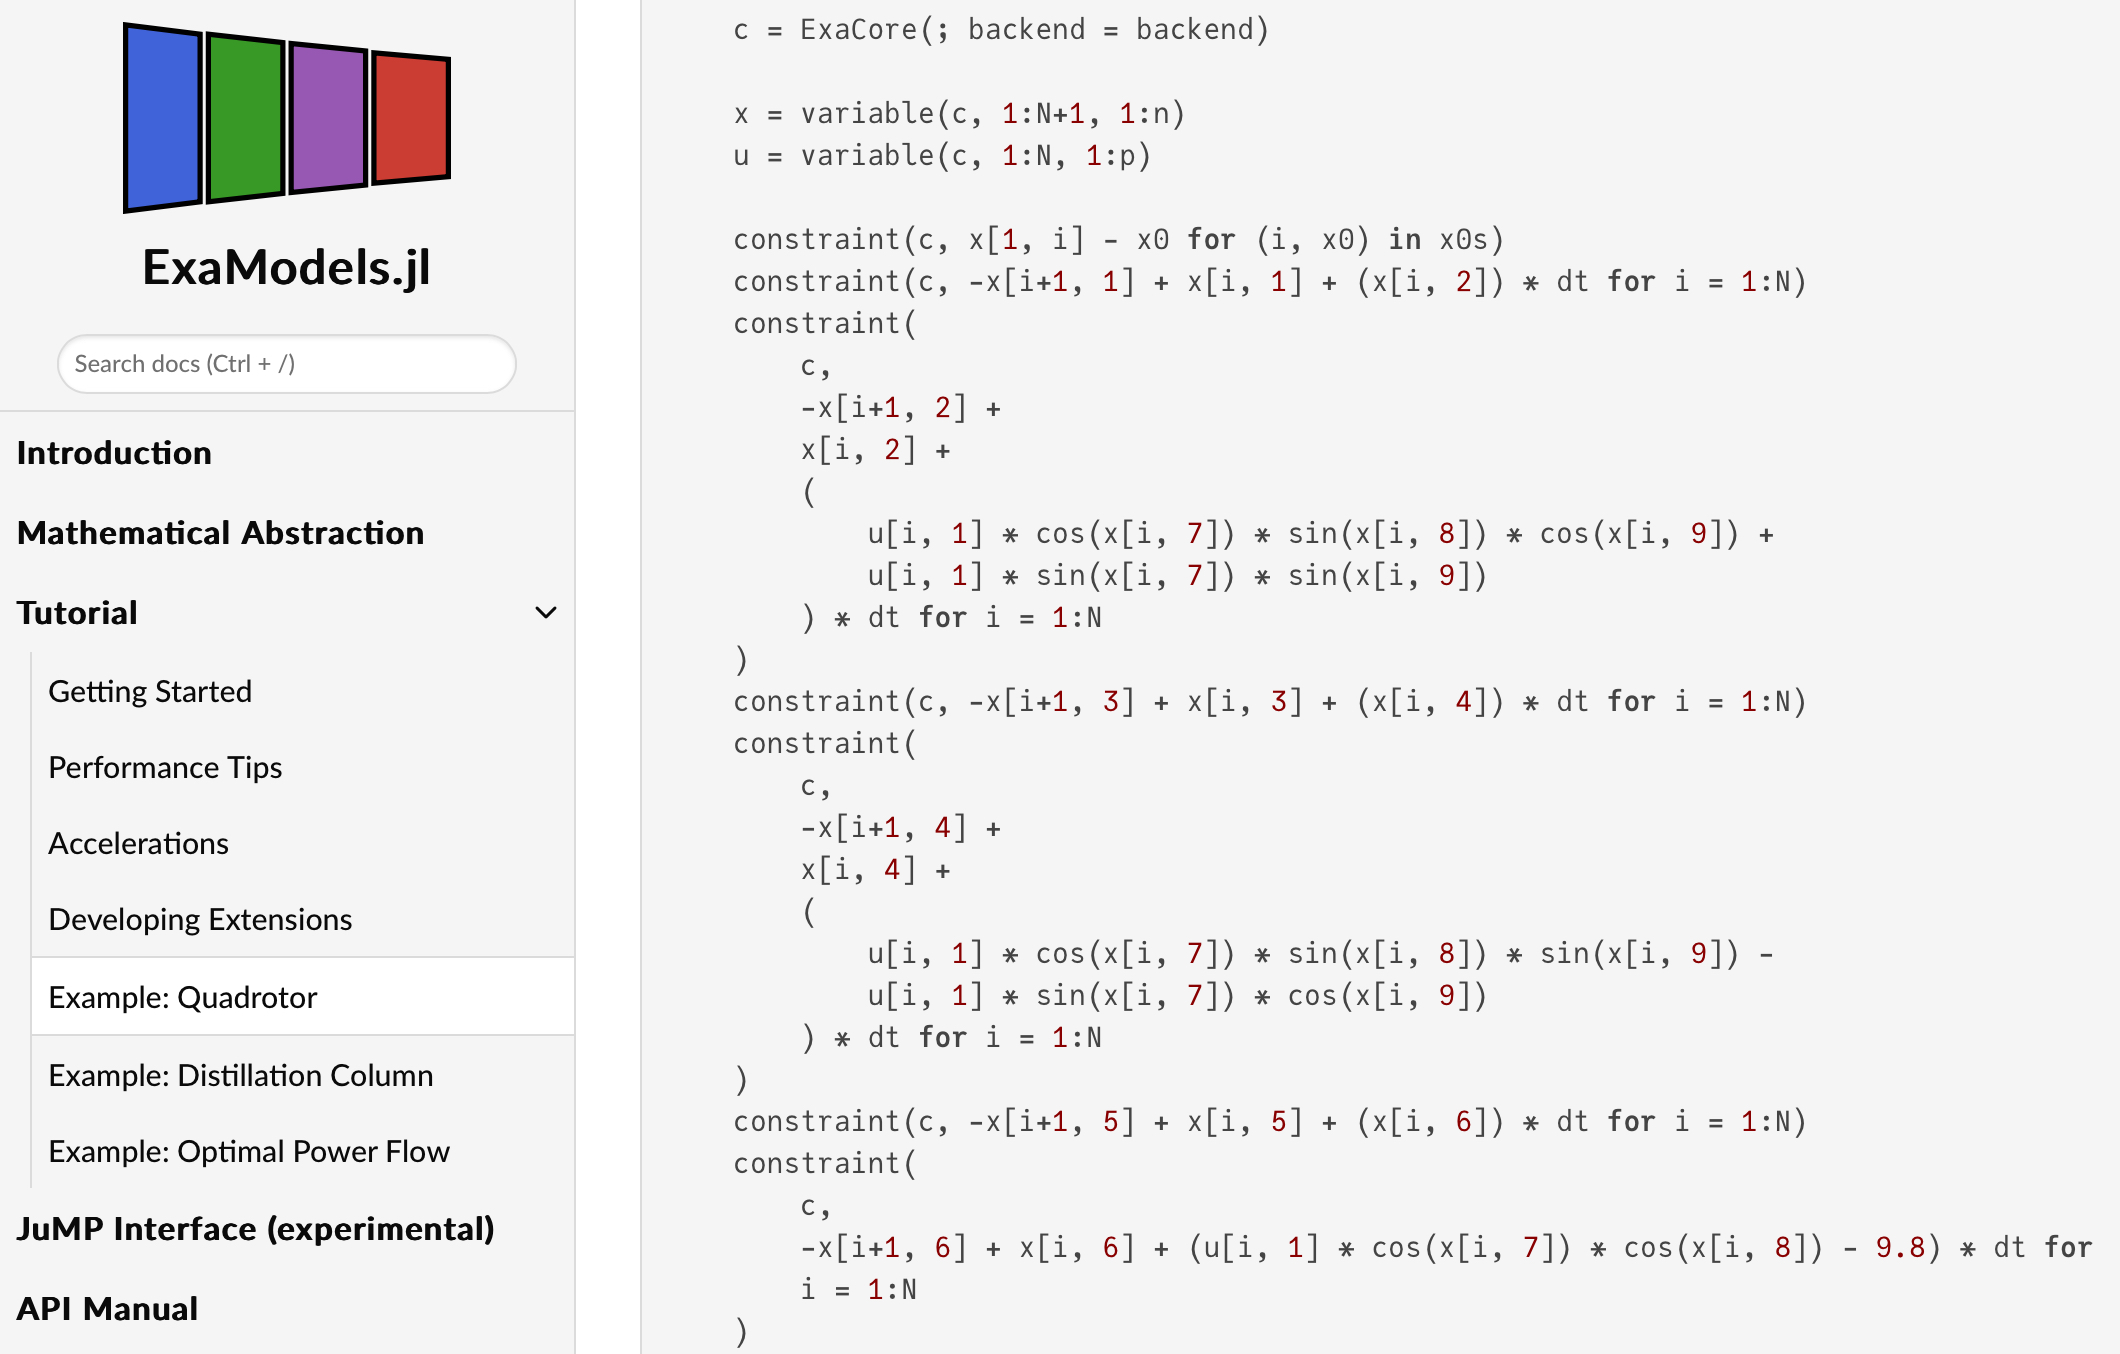
\includegraphics[width=1.0\textwidth]{examodels}

\end{frame}

% Optimisation modellers: infinite dim
\begin{frame}
\frametitle{\bf Optimisation modellers: infinite dim}

\centering 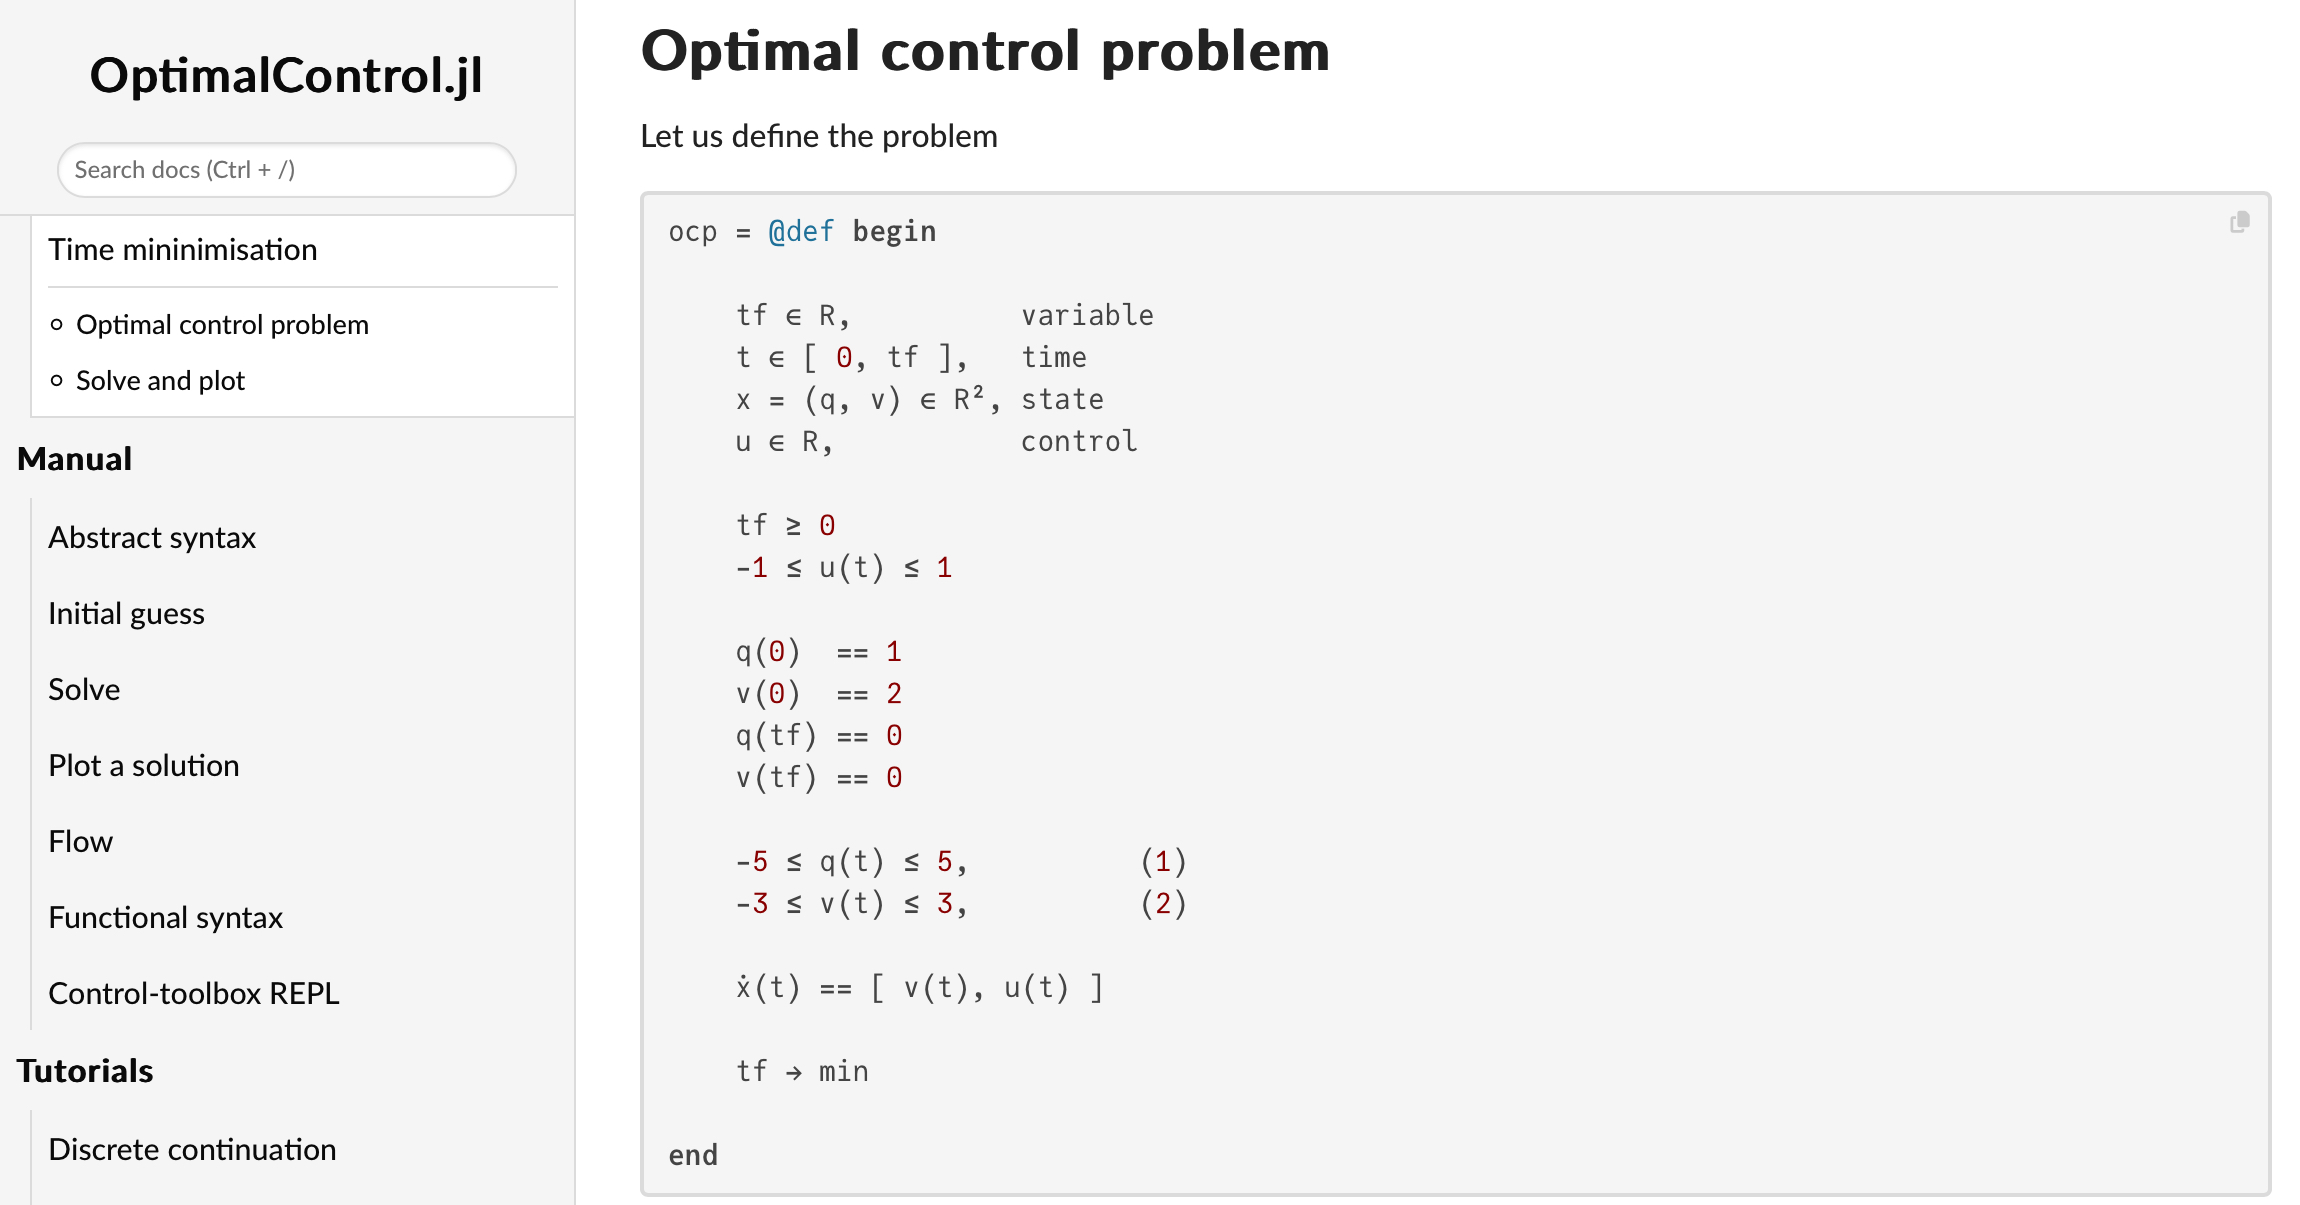
\includegraphics[width=1.05\textwidth]{ct}

\end{frame}

% PEPR IA
\begin{frame}
\frametitle{\bf PEPR IA}

\centering 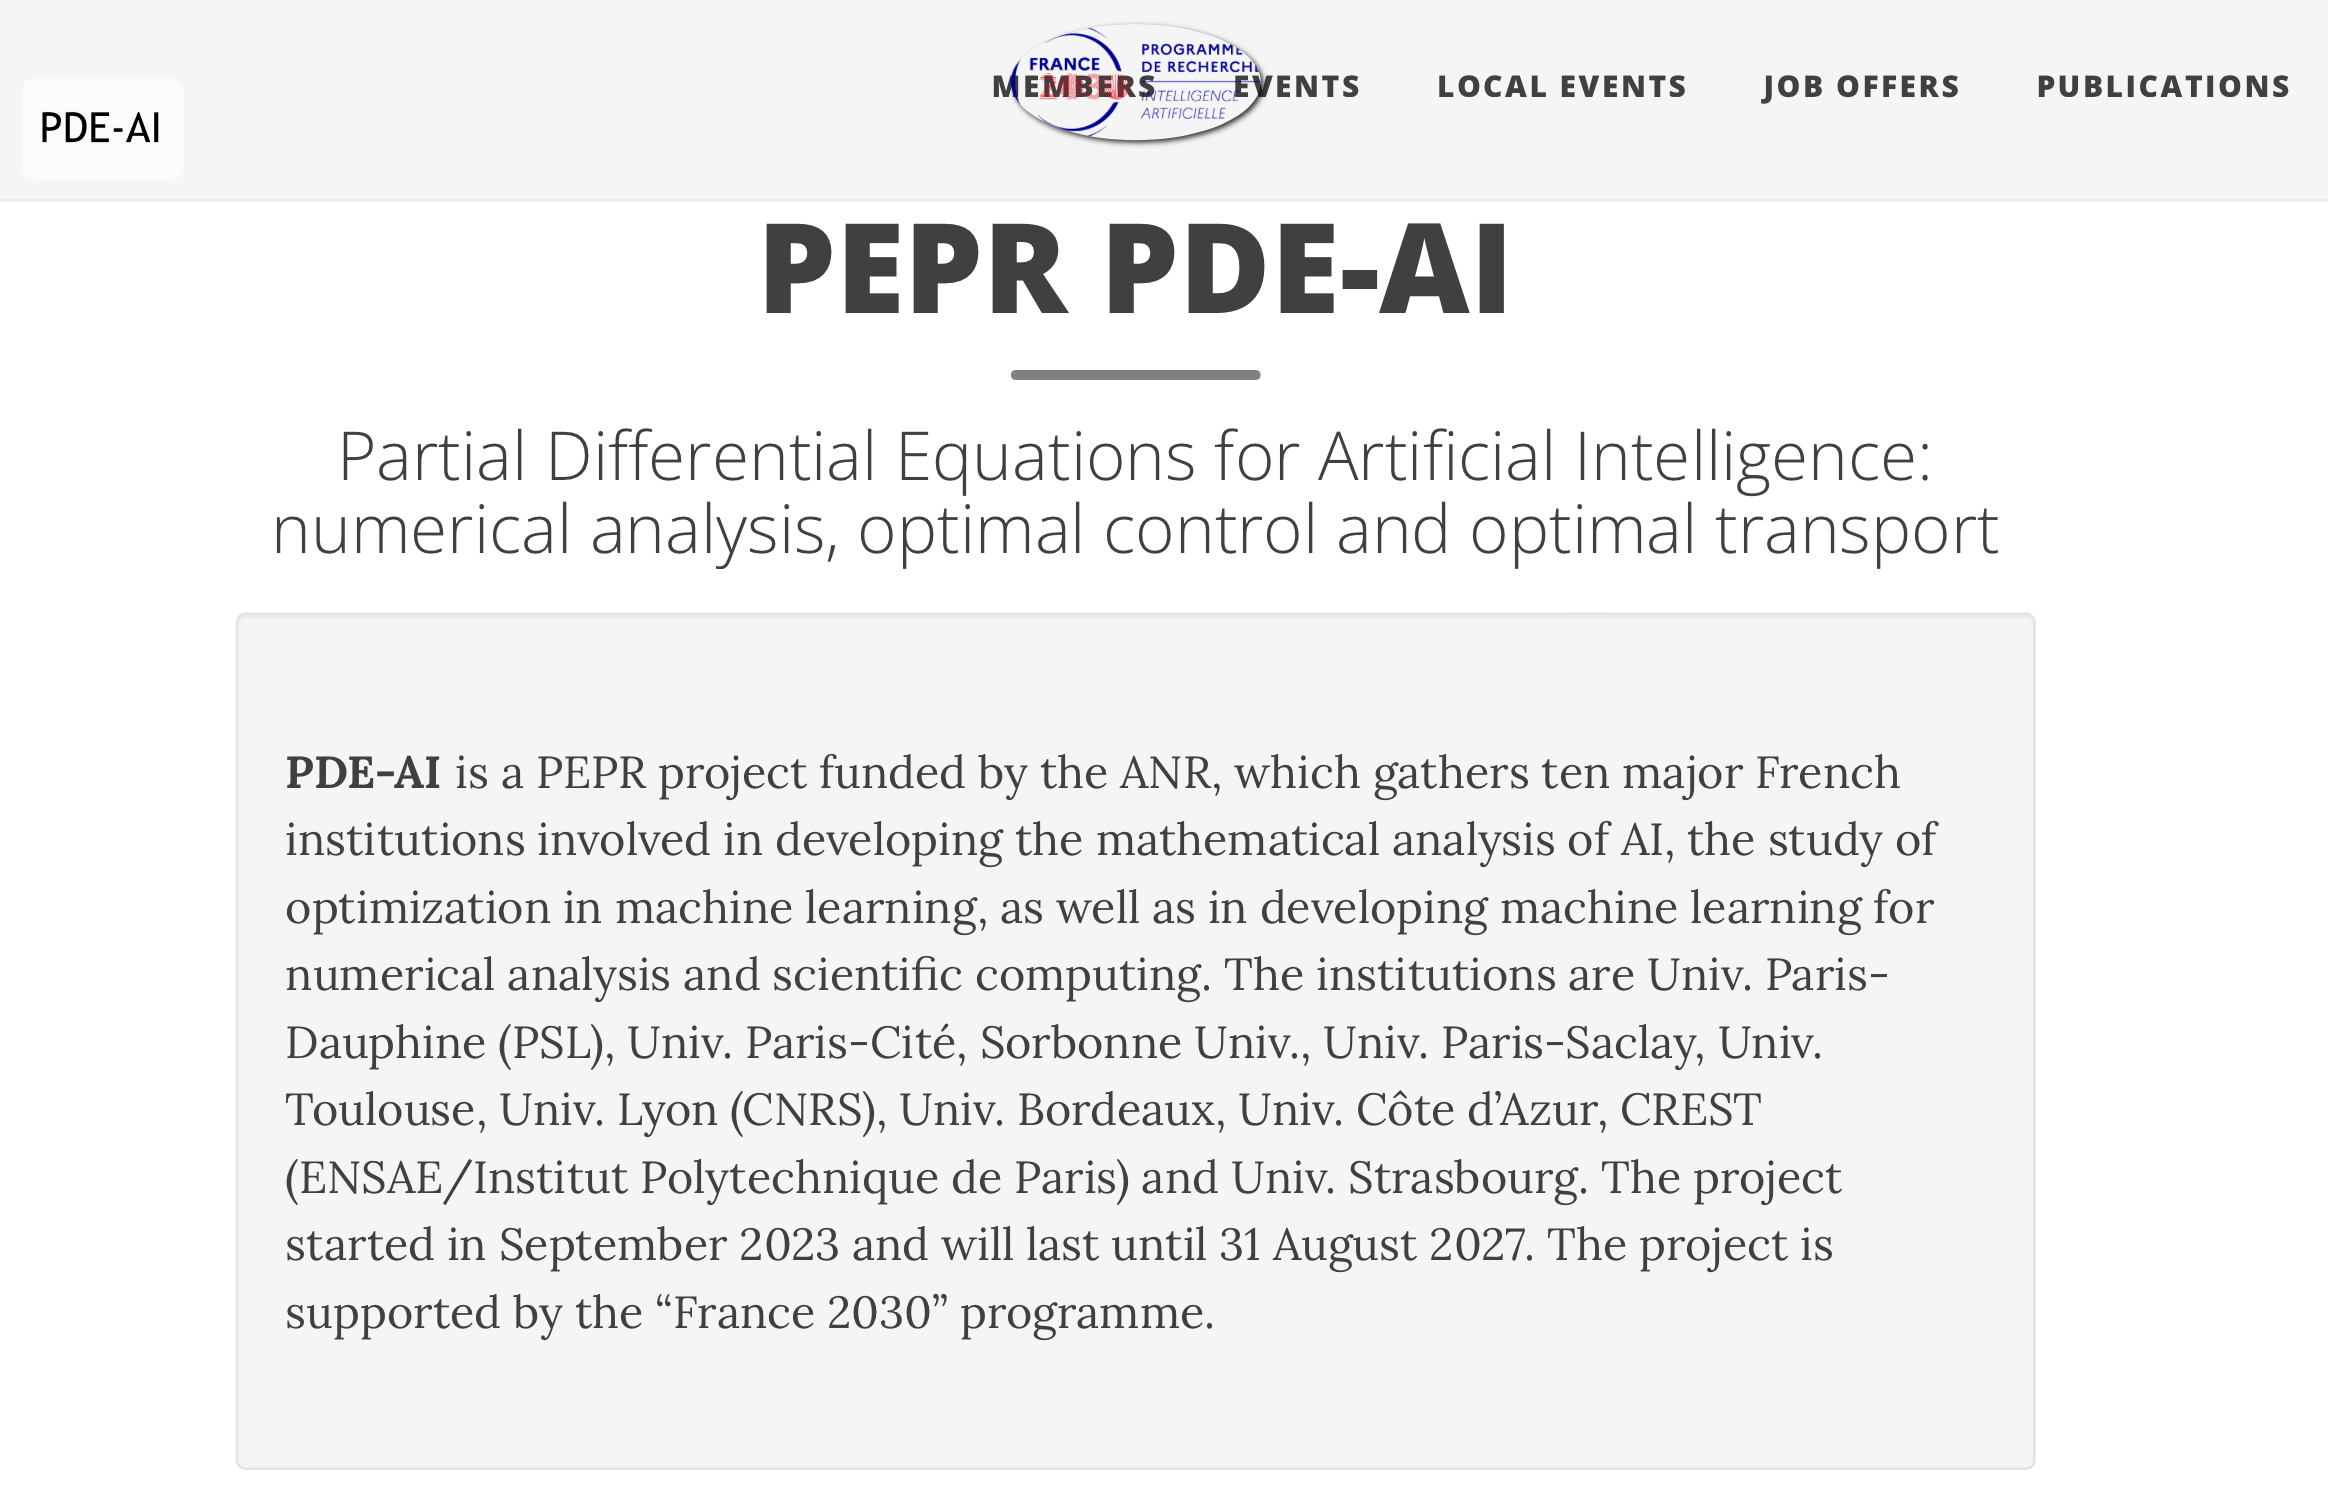
\includegraphics[width=0.99\textwidth]{pdeai}

\begin{itemize} 
\item \href{https://pde-ai.math.cnrs.fr}{pde-ai.math.cnrs.fr}
\end{itemize} 

\end{frame}

\end{document}
